% Options for packages loaded elsewhere
\PassOptionsToPackage{unicode}{hyperref}
\PassOptionsToPackage{hyphens}{url}
\PassOptionsToPackage{dvipsnames,svgnames,x11names}{xcolor}
%
\documentclass[
  letterpaper,
  DIV=11,
  numbers=noendperiod]{scrartcl}

\usepackage{amsmath,amssymb}
\usepackage{iftex}
\ifPDFTeX
  \usepackage[T1]{fontenc}
  \usepackage[utf8]{inputenc}
  \usepackage{textcomp} % provide euro and other symbols
\else % if luatex or xetex
  \usepackage{unicode-math}
  \defaultfontfeatures{Scale=MatchLowercase}
  \defaultfontfeatures[\rmfamily]{Ligatures=TeX,Scale=1}
\fi
\usepackage{lmodern}
\ifPDFTeX\else  
    % xetex/luatex font selection
\fi
% Use upquote if available, for straight quotes in verbatim environments
\IfFileExists{upquote.sty}{\usepackage{upquote}}{}
\IfFileExists{microtype.sty}{% use microtype if available
  \usepackage[]{microtype}
  \UseMicrotypeSet[protrusion]{basicmath} % disable protrusion for tt fonts
}{}
\makeatletter
\@ifundefined{KOMAClassName}{% if non-KOMA class
  \IfFileExists{parskip.sty}{%
    \usepackage{parskip}
  }{% else
    \setlength{\parindent}{0pt}
    \setlength{\parskip}{6pt plus 2pt minus 1pt}}
}{% if KOMA class
  \KOMAoptions{parskip=half}}
\makeatother
\usepackage{xcolor}
\setlength{\emergencystretch}{3em} % prevent overfull lines
\setcounter{secnumdepth}{-\maxdimen} % remove section numbering
% Make \paragraph and \subparagraph free-standing
\makeatletter
\ifx\paragraph\undefined\else
  \let\oldparagraph\paragraph
  \renewcommand{\paragraph}{
    \@ifstar
      \xxxParagraphStar
      \xxxParagraphNoStar
  }
  \newcommand{\xxxParagraphStar}[1]{\oldparagraph*{#1}\mbox{}}
  \newcommand{\xxxParagraphNoStar}[1]{\oldparagraph{#1}\mbox{}}
\fi
\ifx\subparagraph\undefined\else
  \let\oldsubparagraph\subparagraph
  \renewcommand{\subparagraph}{
    \@ifstar
      \xxxSubParagraphStar
      \xxxSubParagraphNoStar
  }
  \newcommand{\xxxSubParagraphStar}[1]{\oldsubparagraph*{#1}\mbox{}}
  \newcommand{\xxxSubParagraphNoStar}[1]{\oldsubparagraph{#1}\mbox{}}
\fi
\makeatother

\usepackage{color}
\usepackage{fancyvrb}
\newcommand{\VerbBar}{|}
\newcommand{\VERB}{\Verb[commandchars=\\\{\}]}
\DefineVerbatimEnvironment{Highlighting}{Verbatim}{commandchars=\\\{\}}
% Add ',fontsize=\small' for more characters per line
\usepackage{framed}
\definecolor{shadecolor}{RGB}{241,243,245}
\newenvironment{Shaded}{\begin{snugshade}}{\end{snugshade}}
\newcommand{\AlertTok}[1]{\textcolor[rgb]{0.68,0.00,0.00}{#1}}
\newcommand{\AnnotationTok}[1]{\textcolor[rgb]{0.37,0.37,0.37}{#1}}
\newcommand{\AttributeTok}[1]{\textcolor[rgb]{0.40,0.45,0.13}{#1}}
\newcommand{\BaseNTok}[1]{\textcolor[rgb]{0.68,0.00,0.00}{#1}}
\newcommand{\BuiltInTok}[1]{\textcolor[rgb]{0.00,0.23,0.31}{#1}}
\newcommand{\CharTok}[1]{\textcolor[rgb]{0.13,0.47,0.30}{#1}}
\newcommand{\CommentTok}[1]{\textcolor[rgb]{0.37,0.37,0.37}{#1}}
\newcommand{\CommentVarTok}[1]{\textcolor[rgb]{0.37,0.37,0.37}{\textit{#1}}}
\newcommand{\ConstantTok}[1]{\textcolor[rgb]{0.56,0.35,0.01}{#1}}
\newcommand{\ControlFlowTok}[1]{\textcolor[rgb]{0.00,0.23,0.31}{\textbf{#1}}}
\newcommand{\DataTypeTok}[1]{\textcolor[rgb]{0.68,0.00,0.00}{#1}}
\newcommand{\DecValTok}[1]{\textcolor[rgb]{0.68,0.00,0.00}{#1}}
\newcommand{\DocumentationTok}[1]{\textcolor[rgb]{0.37,0.37,0.37}{\textit{#1}}}
\newcommand{\ErrorTok}[1]{\textcolor[rgb]{0.68,0.00,0.00}{#1}}
\newcommand{\ExtensionTok}[1]{\textcolor[rgb]{0.00,0.23,0.31}{#1}}
\newcommand{\FloatTok}[1]{\textcolor[rgb]{0.68,0.00,0.00}{#1}}
\newcommand{\FunctionTok}[1]{\textcolor[rgb]{0.28,0.35,0.67}{#1}}
\newcommand{\ImportTok}[1]{\textcolor[rgb]{0.00,0.46,0.62}{#1}}
\newcommand{\InformationTok}[1]{\textcolor[rgb]{0.37,0.37,0.37}{#1}}
\newcommand{\KeywordTok}[1]{\textcolor[rgb]{0.00,0.23,0.31}{\textbf{#1}}}
\newcommand{\NormalTok}[1]{\textcolor[rgb]{0.00,0.23,0.31}{#1}}
\newcommand{\OperatorTok}[1]{\textcolor[rgb]{0.37,0.37,0.37}{#1}}
\newcommand{\OtherTok}[1]{\textcolor[rgb]{0.00,0.23,0.31}{#1}}
\newcommand{\PreprocessorTok}[1]{\textcolor[rgb]{0.68,0.00,0.00}{#1}}
\newcommand{\RegionMarkerTok}[1]{\textcolor[rgb]{0.00,0.23,0.31}{#1}}
\newcommand{\SpecialCharTok}[1]{\textcolor[rgb]{0.37,0.37,0.37}{#1}}
\newcommand{\SpecialStringTok}[1]{\textcolor[rgb]{0.13,0.47,0.30}{#1}}
\newcommand{\StringTok}[1]{\textcolor[rgb]{0.13,0.47,0.30}{#1}}
\newcommand{\VariableTok}[1]{\textcolor[rgb]{0.07,0.07,0.07}{#1}}
\newcommand{\VerbatimStringTok}[1]{\textcolor[rgb]{0.13,0.47,0.30}{#1}}
\newcommand{\WarningTok}[1]{\textcolor[rgb]{0.37,0.37,0.37}{\textit{#1}}}

\providecommand{\tightlist}{%
  \setlength{\itemsep}{0pt}\setlength{\parskip}{0pt}}\usepackage{longtable,booktabs,array}
\usepackage{calc} % for calculating minipage widths
% Correct order of tables after \paragraph or \subparagraph
\usepackage{etoolbox}
\makeatletter
\patchcmd\longtable{\par}{\if@noskipsec\mbox{}\fi\par}{}{}
\makeatother
% Allow footnotes in longtable head/foot
\IfFileExists{footnotehyper.sty}{\usepackage{footnotehyper}}{\usepackage{footnote}}
\makesavenoteenv{longtable}
\usepackage{graphicx}
\makeatletter
\newsavebox\pandoc@box
\newcommand*\pandocbounded[1]{% scales image to fit in text height/width
  \sbox\pandoc@box{#1}%
  \Gscale@div\@tempa{\textheight}{\dimexpr\ht\pandoc@box+\dp\pandoc@box\relax}%
  \Gscale@div\@tempb{\linewidth}{\wd\pandoc@box}%
  \ifdim\@tempb\p@<\@tempa\p@\let\@tempa\@tempb\fi% select the smaller of both
  \ifdim\@tempa\p@<\p@\scalebox{\@tempa}{\usebox\pandoc@box}%
  \else\usebox{\pandoc@box}%
  \fi%
}
% Set default figure placement to htbp
\def\fps@figure{htbp}
\makeatother

\KOMAoption{captions}{tableheading}
\makeatletter
\@ifpackageloaded{caption}{}{\usepackage{caption}}
\AtBeginDocument{%
\ifdefined\contentsname
  \renewcommand*\contentsname{Table of contents}
\else
  \newcommand\contentsname{Table of contents}
\fi
\ifdefined\listfigurename
  \renewcommand*\listfigurename{List of Figures}
\else
  \newcommand\listfigurename{List of Figures}
\fi
\ifdefined\listtablename
  \renewcommand*\listtablename{List of Tables}
\else
  \newcommand\listtablename{List of Tables}
\fi
\ifdefined\figurename
  \renewcommand*\figurename{Figure}
\else
  \newcommand\figurename{Figure}
\fi
\ifdefined\tablename
  \renewcommand*\tablename{Table}
\else
  \newcommand\tablename{Table}
\fi
}
\@ifpackageloaded{float}{}{\usepackage{float}}
\floatstyle{ruled}
\@ifundefined{c@chapter}{\newfloat{codelisting}{h}{lop}}{\newfloat{codelisting}{h}{lop}[chapter]}
\floatname{codelisting}{Listing}
\newcommand*\listoflistings{\listof{codelisting}{List of Listings}}
\makeatother
\makeatletter
\makeatother
\makeatletter
\@ifpackageloaded{caption}{}{\usepackage{caption}}
\@ifpackageloaded{subcaption}{}{\usepackage{subcaption}}
\makeatother

\usepackage{bookmark}

\IfFileExists{xurl.sty}{\usepackage{xurl}}{} % add URL line breaks if available
\urlstyle{same} % disable monospaced font for URLs
\hypersetup{
  pdftitle={Survival Analysis with the deidentified Thyroid Cancer Dataset},
  pdfauthor={RPythonStudyGroup feat. ChatGPT},
  colorlinks=true,
  linkcolor={blue},
  filecolor={Maroon},
  citecolor={Blue},
  urlcolor={Blue},
  pdfcreator={LaTeX via pandoc}}


\title{Survival Analysis with the deidentified Thyroid Cancer Dataset}
\author{RPythonStudyGroup feat. ChatGPT}
\date{2025-02-03}

\begin{document}
\maketitle


\subsection{준비하기}\label{uxc900uxbe44uxd558uxae30}

\subsubsection{git clone}\label{git-clone}

\begin{itemize}
\tightlist
\item
  원격저장소 HTTP url:
  https://github.com/RPythonGroup/Survival\_Exercise.git
\item
  터미널에서 git clone 시 현재 디렉토리 하부에 지정하는 디렉토리명으로
  clone 됨.
\end{itemize}

\begin{Shaded}
\begin{Highlighting}[]
\FunctionTok{git}\NormalTok{ clone https://github.com/RPythonGroup/Survival\_Exercise.git R441{-}Survival\_Exercise}
\end{Highlighting}
\end{Shaded}

\begin{itemize}
\tightlist
\item
  RStudio 프로젝트만들기에서 기존 디렉토리에서 만들기에서 clone 된
  디렉토리를 선택하면 됨.
\item
  패키지관리를 renv로 할려면,

  \begin{itemize}
  \item
\begin{verbatim}
  renv::activate로 활성화시키고,
\end{verbatim}
  \item
\begin{verbatim}
  renv::snapshot 으로 renv.lock 파일의 패키지 목록을 설치하도록 옵션을 선택하시면 됨. 
\end{verbatim}
  \item
\begin{verbatim}
  설치가 완료되면 renv::status() 로 프로젝트에 설치된 패키지와 renv.lock 파일에 기록된 패키지 목록이 일치하는지 확인하면 됨.
\end{verbatim}
  \end{itemize}
\end{itemize}

\subsubsection{readRDS}\label{readrds}

\begin{itemize}
\tightlist
\item
  R에서만 사용하는 자료형태인 RDS를 읽어오며, 자료형이 보전되고 빠름
\end{itemize}

\begin{Shaded}
\begin{Highlighting}[]
\FunctionTok{library}\NormalTok{(dplyr)}
\end{Highlighting}
\end{Shaded}

\begin{verbatim}

Attaching package: 'dplyr'
\end{verbatim}

\begin{verbatim}
The following objects are masked from 'package:stats':

    filter, lag
\end{verbatim}

\begin{verbatim}
The following objects are masked from 'package:base':

    intersect, setdiff, setequal, union
\end{verbatim}

\begin{Shaded}
\begin{Highlighting}[]
\NormalTok{rai\_recur }\OtherTok{\textless{}{-}} \FunctionTok{readRDS}\NormalTok{(}\StringTok{"deidentified\_data/rai\_recur.rds"}\NormalTok{)}
\end{Highlighting}
\end{Shaded}

\subsubsection{mytable}\label{mytable}

\begin{itemize}
\tightlist
\item
  mytable로 자료 개요 파악
\item
  mylatex 출력은 성공하지 못함.
\end{itemize}

\begin{Shaded}
\begin{Highlighting}[]
\FunctionTok{library}\NormalTok{(moonBook)}

\CommentTok{\# mytable(recur\textasciitilde{}.,data=rai\_recur) \%\textgreater{}\% mylatex() \%\textgreater{}\% cat \# 정상작동이 되지 않는 이유는?}

\FunctionTok{mytable}\NormalTok{(recur}\SpecialCharTok{\textasciitilde{}}\NormalTok{.,}\AttributeTok{data=}\NormalTok{rai\_recur)}
\end{Highlighting}
\end{Shaded}

\begin{verbatim}

                     Descriptive Statistics by 'recur'                    
——————————————————————————————————————————————————————————————————————————— 
                                      FALSE               TRUE          p  
                                     (N=1097)            (N=83)      
——————————————————————————————————————————————————————————————————————————— 
 pt_id                          unique values:1179 unique values:1179      
 age                               48.2 ± 10.9        42.4 ± 12.5     0.000
 sex                                                                  0.001
   - F                             881 (80.3%)         53 (63.9%)          
   - M                             216 (19.7%)         30 (36.1%)          
 op_year                          2012.2 ±  5.4      2008.6 ±  6.2    0.000
 surgeon                                                              0.000
   - CIJ                            72 ( 6.6%)         1 ( 1.2%)           
   - GS                             19 ( 1.7%)         3 ( 3.6%)           
   - KCCH                           61 ( 5.6%)         2 ( 2.4%)           
   - LBC                           104 ( 9.5%)         6 ( 7.2%)           
   - LGH                           447 (40.7%)         29 (34.9%)          
   - LMC                           226 (20.6%)         8 ( 9.6%)           
   - LYS                            25 ( 2.3%)         5 ( 6.0%)           
   - OKK                            4 ( 0.4%)          2 ( 2.4%)           
   - outside                        63 ( 5.7%)         23 (27.7%)          
   - SYS                            76 ( 6.9%)         4 ( 4.8%)           
 Thyroidectomy_Type                                                   0.551
   - Lobectomy_Completion           64 ( 5.8%)         3 ( 3.6%)           
   - TT                            1033 (94.2%)        80 (96.4%)          
 ND_Type                                                              0.001
   - CND                           833 (75.9%)         45 (54.2%)          
   - FND                            9 ( 0.8%)          2 ( 2.4%)           
   - mRND                           2 ( 0.2%)          1 ( 1.2%)           
   - ND                             76 ( 6.9%)         10 (12.0%)          
   - Not Done                       37 ( 3.4%)         4 ( 4.8%)           
   - Picking                        7 ( 0.6%)          1 ( 1.2%)           
   - SND                           133 (12.1%)         20 (24.1%)          
 Risk                                                                 0.000
   - High                          178 (16.2%)         34 (41.0%)          
   - Intermediate                  535 (48.8%)         43 (51.8%)          
   - Low                           384 (35.0%)         6 ( 7.2%)           
 histology                                                            0.264
   - FTC                            24 ( 2.2%)          0 ( 0.0%)          
   - HTC                            2 ( 0.2%)          1 ( 1.2%)           
   - Mixed                          1 ( 0.1%)           0 ( 0.0%)          
   - PDTC                           2 ( 0.2%)           0 ( 0.0%)          
   - PTC                           1068 (97.4%)        82 (98.8%)          
 subtype                                                              0.065
   - clear_cell                     1 ( 0.1%)           0 ( 0.0%)          
   - conventional                  982 (89.5%)         79 (95.2%)          
   - cribriform-morular             1 ( 0.1%)           0 ( 0.0%)          
   - diffuse_sclerosing             5 ( 0.5%)          3 ( 3.6%)           
   - encapsulated_angioinvasive     4 ( 0.4%)           0 ( 0.0%)          
   - follicular                     60 ( 5.5%)          0 ( 0.0%)          
   - minimally_invasive             20 ( 1.8%)          0 ( 0.0%)          
   - oncocytic                      3 ( 0.3%)           0 ( 0.0%)          
   - poorly_differentiated          1 ( 0.1%)           0 ( 0.0%)          
   - solid                          3 ( 0.3%)           0 ( 0.0%)          
   - tall_cell                      16 ( 1.5%)         1 ( 1.2%)           
   - widely_invasive                1 ( 0.1%)           0 ( 0.0%)          
 pT                                                                   0.000
   - T1a                           486 (44.3%)         13 (15.7%)          
   - T1b                           387 (35.3%)         28 (33.7%)          
   - T2                            115 (10.5%)         19 (22.9%)          
   - T3a                            24 ( 2.2%)         6 ( 7.2%)           
   - T3b                            59 ( 5.4%)         6 ( 7.2%)           
   - T4a                            26 ( 2.4%)         10 (12.0%)          
   - T4b                             0 ( 0.0%)         1 ( 1.2%)           
 size                               1.3 ±  0.9         2.2 ±  1.7     0.000
 Multiplicity                                                         0.226
   - Multiple                      565 (51.5%)         49 (59.0%)          
   - Single                        532 (48.5%)         34 (41.0%)          
 ETE                                                                  0.142
   - N                             357 (32.5%)         20 (24.1%)          
   - Y                             740 (67.5%)         63 (75.9%)          
 gross_ETE                                                            0.000
   - N                             1017 (92.7%)        67 (80.7%)          
   - Y                              80 ( 7.3%)         16 (19.3%)          
 pN                                                                   0.000
   - N0                            335 (30.5%)         9 (10.8%)           
   - N1a                           499 (45.5%)         39 (47.0%)          
   - N1b                           205 (18.7%)         31 (37.3%)          
   - Nx                             58 ( 5.3%)         4 ( 4.8%)           
 ENE                                                                  0.001
   - N                             985 (89.8%)         64 (77.1%)          
   - Y                             112 (10.2%)         19 (22.9%)          
 time                              143.4 ± 65.0       53.0 ± 53.0     0.000
——————————————————————————————————————————————————————————————————————————— 
\end{verbatim}

\subsection{Surv함수}\label{survuxd568uxc218}

\begin{itemize}
\tightlist
\item
  time과 event를 인자로 받아 특수한 형태의 matrix인 생존(survival) 객체
  반환
\end{itemize}

\begin{Shaded}
\begin{Highlighting}[]
\FunctionTok{library}\NormalTok{(survival)}

\NormalTok{rai\_recur}\SpecialCharTok{$}\NormalTok{recur }\OtherTok{\textless{}{-}} \FunctionTok{as.integer}\NormalTok{(rai\_recur}\SpecialCharTok{$}\NormalTok{recur)}
\NormalTok{km }\OtherTok{\textless{}{-}} \FunctionTok{Surv}\NormalTok{(rai\_recur}\SpecialCharTok{$}\NormalTok{time, }\AttributeTok{event =}\NormalTok{ rai\_recur}\SpecialCharTok{$}\NormalTok{recur) }\DocumentationTok{\#\# default type : "right"}
\CommentTok{\# km \textless{}{-} Surv(time=time, event = recur, data=rai\_recur) \# data= 형식을 지원하지 않음}

\FunctionTok{str}\NormalTok{(km)}
\end{Highlighting}
\end{Shaded}

\begin{verbatim}
 'Surv' num [1:1180, 1:2] 387+ 124+ 176+ 113+ 242+  42+ 209+ 159+ 167+ 416+ ...
 - attr(*, "dimnames")=List of 2
  ..$ : NULL
  ..$ : chr [1:2] "time" "status"
 - attr(*, "type")= chr "right"
\end{verbatim}

\begin{Shaded}
\begin{Highlighting}[]
\FunctionTok{head}\NormalTok{(km)}
\end{Highlighting}
\end{Shaded}

\begin{verbatim}
[1] 387+ 124+ 176+ 113+ 242+  42+
\end{verbatim}

\subsubsection{plot}\label{plot}

\begin{itemize}
\tightlist
\item
  plot() 함수는 제네릭 함수로, 기본적으로 산점도를 그리지만, Surv 객체를
  인자로 받으면 내부적으로 plot.survfit() method를 호출하여
  Kaplan-Meier(KM) 곡선을 반환함
\item
  time의 단위가 월이라서 x 축은 400까지 표시됨
\end{itemize}

\begin{Shaded}
\begin{Highlighting}[]
\FunctionTok{plot}\NormalTok{(km) }\DocumentationTok{\#\# km {-} Surv class (time, status) 가지고 있는 리스트}
\end{Highlighting}
\end{Shaded}

\pandocbounded{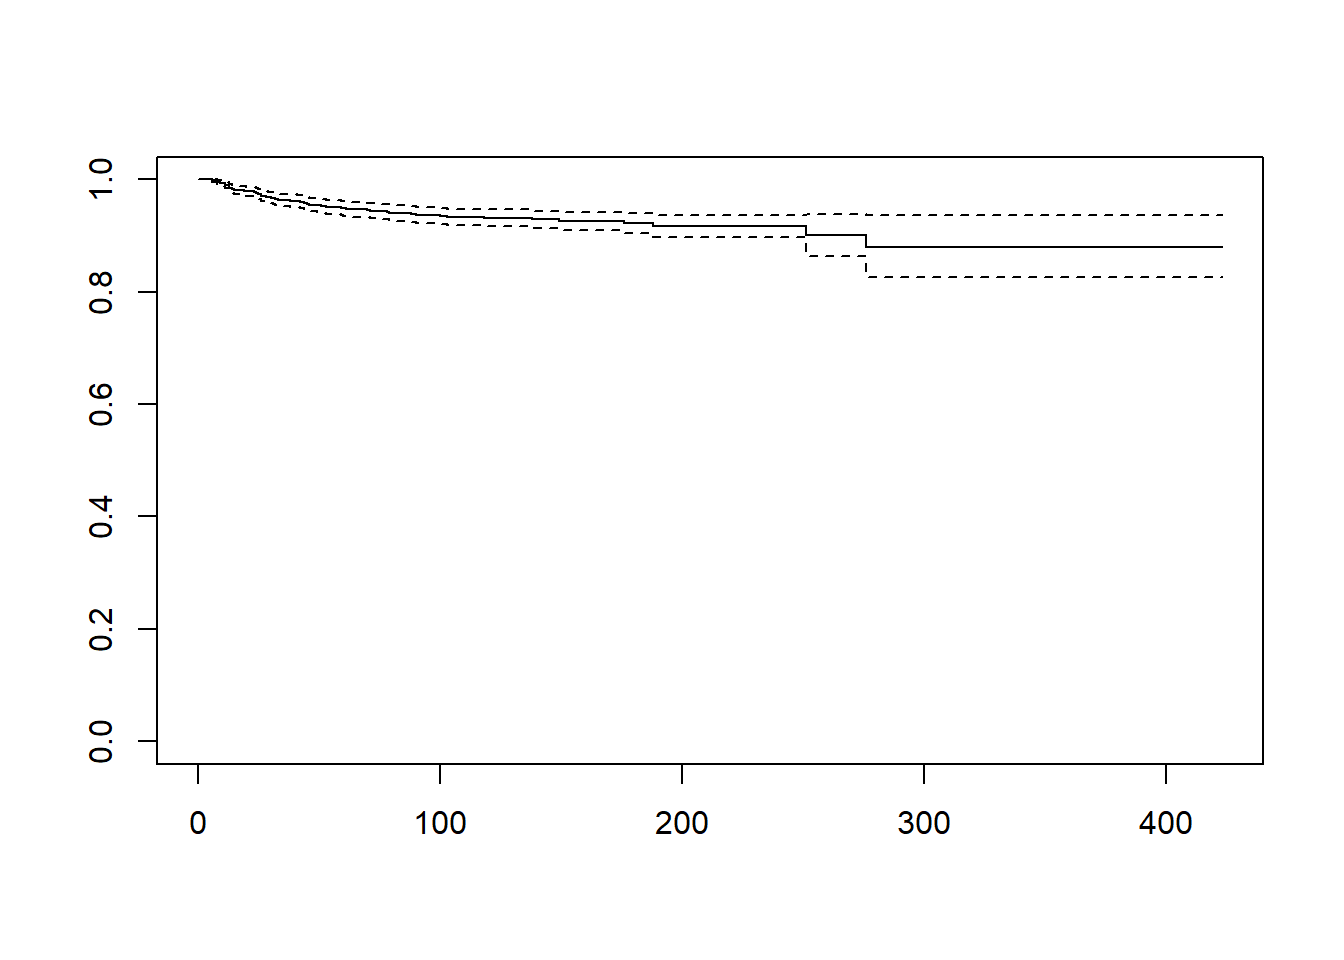
\includegraphics[keepaspectratio]{index_files/figure-pdf/plot.survfit-1.pdf}}

\begin{itemize}
\tightlist
\item
  Surv 객체는 \textbf{survfit 함수의 인자}로 사용되므로 중요
\end{itemize}

\subsubsection{중앙값
생존기간}\label{uxc911uxc559uxac12-uxc0dduxc874uxae30uxac04}

\begin{itemize}
\tightlist
\item
  50\%에 도달하지 못하여 NA 반환됨
\end{itemize}

\begin{Shaded}
\begin{Highlighting}[]
\FunctionTok{median}\NormalTok{(km)  }\DocumentationTok{\#\# Surv 객체에 대한 method 함수들이 있다.}
\end{Highlighting}
\end{Shaded}

\begin{verbatim}
$quantile
50 
NA 

$lower
50 
NA 

$upper
50 
NA 
\end{verbatim}

\subsubsection{평균생존기간}\label{uxd3c9uxade0uxc0dduxc874uxae30uxac04}

\begin{itemize}
\tightlist
\item
  데이터셋의 time 변수는 입력단위가 월이므로 재발에 소요된 평균이 약
  69개월 ?
\end{itemize}

\begin{Shaded}
\begin{Highlighting}[]
\FunctionTok{mean}\NormalTok{(km)}
\end{Highlighting}
\end{Shaded}

\begin{verbatim}
[1] 68.56186
\end{verbatim}

\subsection{survfit}\label{survfit}

\begin{itemize}
\tightlist
\item
  Surv 객체와 공변량을 formula 형태의 인자로 받아 Kaplan-Meier 또는 Cox
  모델 기반 생존 확률을 저장한 객체를 반환
\end{itemize}

\subsubsection{Kaplan-Meier 기반}\label{kaplan-meier-uxae30uxbc18}

\begin{Shaded}
\begin{Highlighting}[]
\FunctionTok{plot}\NormalTok{(}\FunctionTok{survfit}\NormalTok{(km}\SpecialCharTok{\textasciitilde{}}\DecValTok{1}\NormalTok{)) }\CommentTok{\#Kaplan{-}Meier 기반}
\end{Highlighting}
\end{Shaded}

\pandocbounded{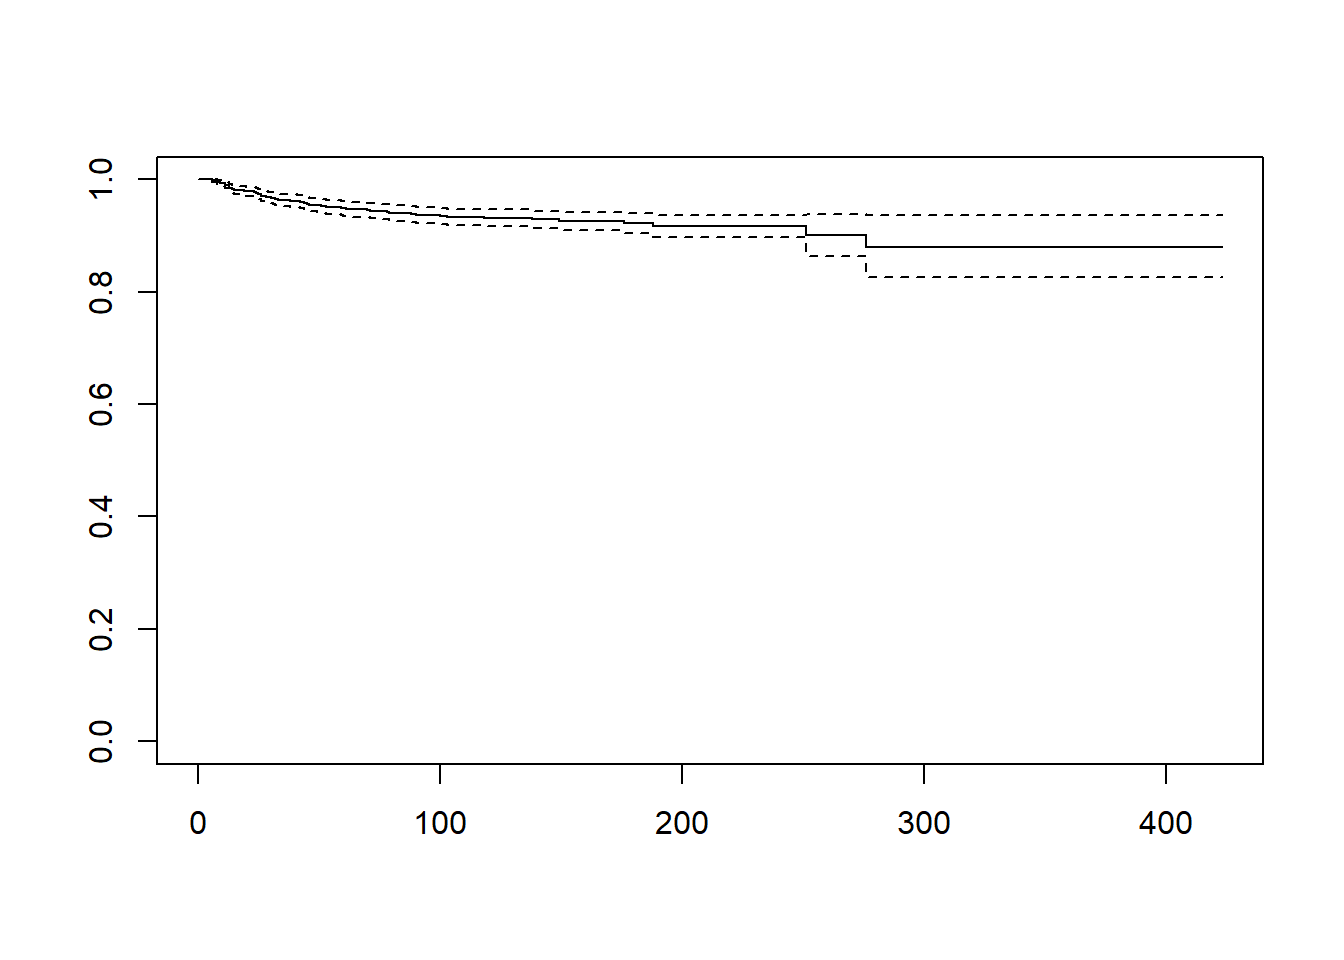
\includegraphics[keepaspectratio]{index_files/figure-pdf/plot_survfit-1.pdf}}

\subsubsection{cox model 기반}\label{cox-model-uxae30uxbc18}

\begin{Shaded}
\begin{Highlighting}[]
\NormalTok{km\_fit }\OtherTok{\textless{}{-}} \FunctionTok{survfit}\NormalTok{(km}\SpecialCharTok{\textasciitilde{}}\NormalTok{rai\_recur}\SpecialCharTok{$}\NormalTok{sex) }\CommentTok{\#cox model 기반}

\FunctionTok{plot}\NormalTok{(km\_fit)}
\end{Highlighting}
\end{Shaded}

\pandocbounded{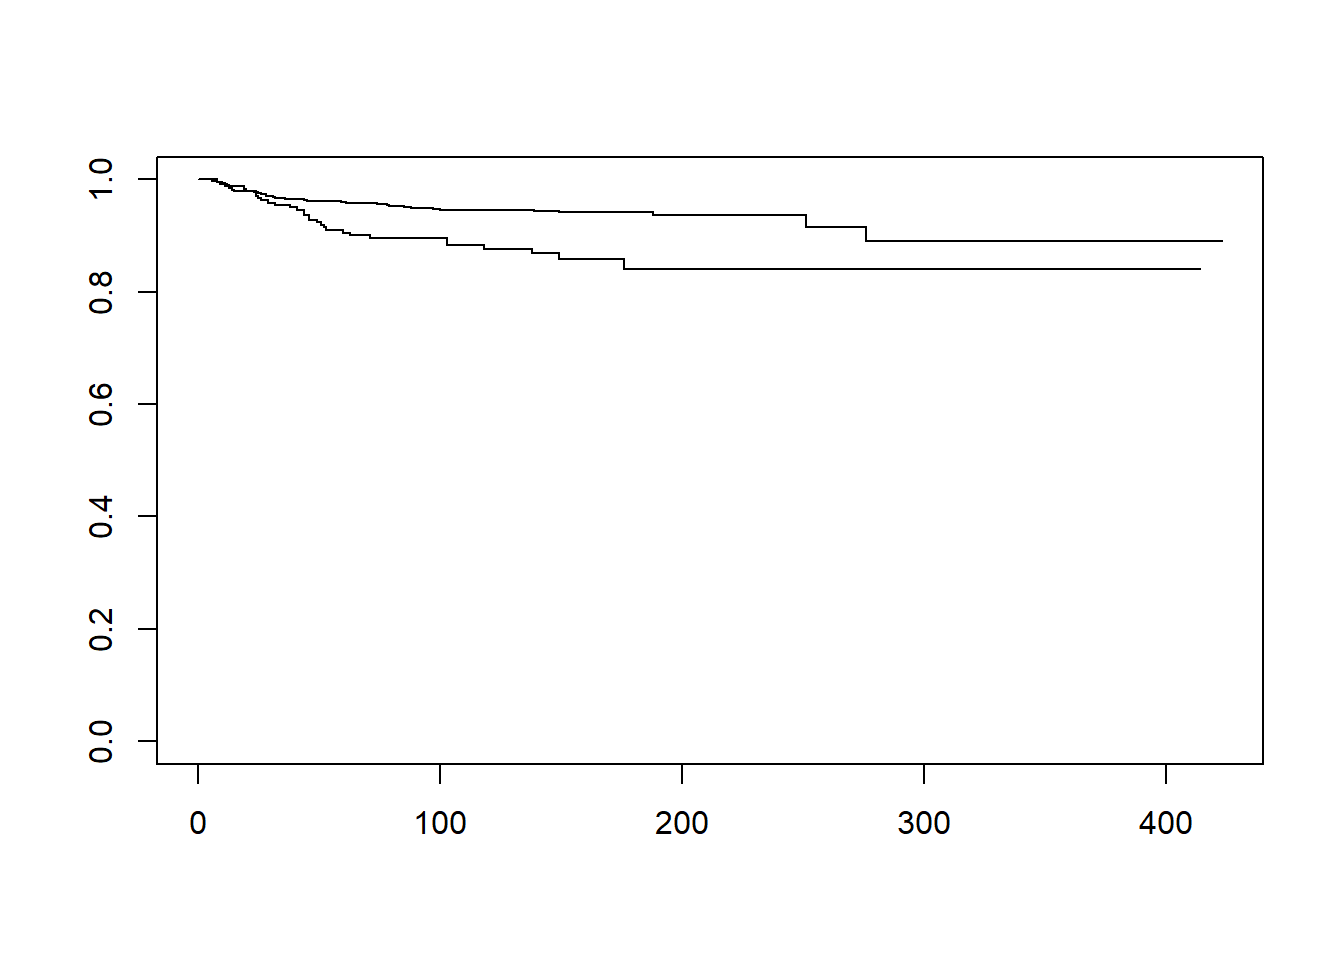
\includegraphics[keepaspectratio]{index_files/figure-pdf/plot_cox-1.pdf}}

\subsubsection{summary}\label{summary}

\begin{Shaded}
\begin{Highlighting}[]
\FunctionTok{summary}\NormalTok{(km\_fit) }
\end{Highlighting}
\end{Shaded}

\begin{verbatim}
Call: survfit(formula = km ~ rai_recur$sex)

                rai_recur$sex=F 
 time n.risk n.event survival std.err lower 95% CI upper 95% CI
    6    934       2    0.998 0.00151        0.995        1.000
    8    932       2    0.996 0.00214        0.992        1.000
    9    930       1    0.995 0.00239        0.990        0.999
   10    929       1    0.994 0.00261        0.988        0.999
   11    928       2    0.991 0.00302        0.986        0.997
   12    926       1    0.990 0.00320        0.984        0.997
   13    925       5    0.985 0.00398        0.977        0.993
   14    920       3    0.982 0.00437        0.973        0.990
   15    917       2    0.980 0.00462        0.971        0.989
   17    915       1    0.979 0.00474        0.969        0.988
   23    902       1    0.978 0.00485        0.968        0.987
   25    898       2    0.975 0.00508        0.965        0.985
   26    895       2    0.973 0.00530        0.963        0.984
   28    888       2    0.971 0.00551        0.960        0.982
   30    883       1    0.970 0.00561        0.959        0.981
   31    880       1    0.969 0.00571        0.958        0.980
   32    878       1    0.968 0.00581        0.956        0.979
   33    876       1    0.967 0.00591        0.955        0.978
   36    868       1    0.965 0.00601        0.954        0.977
   42    850       1    0.964 0.00611        0.952        0.976
   44    846       1    0.963 0.00620        0.951        0.975
   45    844       1    0.962 0.00630        0.950        0.974
   57    820       1    0.961 0.00640        0.948        0.973
   59    816       1    0.960 0.00650        0.947        0.972
   61    804       1    0.958 0.00660        0.946        0.971
   70    787       1    0.957 0.00670        0.944        0.970
   74    767       1    0.956 0.00681        0.943        0.969
   78    762       1    0.955 0.00692        0.941        0.968
   79    759       2    0.952 0.00712        0.938        0.966
   85    753       1    0.951 0.00722        0.937        0.965
   88    745       1    0.950 0.00733        0.935        0.964
   90    740       1    0.948 0.00743        0.934        0.963
   97    720       1    0.947 0.00753        0.932        0.962
  100    710       1    0.946 0.00764        0.931        0.961
  139    510       1    0.944 0.00785        0.929        0.959
  149    436       1    0.942 0.00812        0.926        0.958
  188    161       1    0.936 0.00996        0.917        0.956
  251     47       1    0.916 0.02198        0.874        0.960
  276     35       1    0.890 0.03348        0.827        0.958

                rai_recur$sex=M 
 time n.risk n.event survival std.err lower 95% CI upper 95% CI
    8    246       1    0.996 0.00406        0.988        1.000
    9    245       1    0.992 0.00573        0.981        1.000
   11    244       1    0.988 0.00700        0.974        1.000
   19    242       1    0.984 0.00807        0.968        1.000
   20    240       1    0.980 0.00902        0.962        0.997
   24    234       2    0.971 0.01071        0.950        0.992
   25    232       1    0.967 0.01145        0.945        0.990
   26    231       1    0.963 0.01214        0.939        0.987
   29    228       1    0.959 0.01280        0.934        0.984
   32    225       1    0.954 0.01344        0.928        0.981
   38    219       1    0.950 0.01407        0.923        0.978
   41    218       1    0.946 0.01466        0.917        0.975
   44    216       2    0.937 0.01578        0.907        0.968
   46    212       2    0.928 0.01682        0.896        0.962
   49    206       1    0.924 0.01733        0.890        0.958
   51    204       1    0.919 0.01783        0.885        0.955
   52    203       1    0.915 0.01831        0.879        0.951
   53    201       1    0.910 0.01877        0.874        0.948
   60    188       1    0.905 0.01929        0.868        0.944
   63    183       1    0.900 0.01981        0.862        0.940
   71    168       1    0.895 0.02040        0.856        0.936
  103    145       2    0.882 0.02191        0.841        0.926
  118    133       1    0.876 0.02272        0.832        0.922
  138    116       1    0.868 0.02375        0.823        0.916
  149     92       1    0.859 0.02530        0.811        0.910
  176     46       1    0.840 0.03088        0.782        0.903
\end{verbatim}

\subsubsection{summary 기간지정}\label{summary-uxae30uxac04uxc9c0uxc815}

\begin{Shaded}
\begin{Highlighting}[]
\FunctionTok{summary}\NormalTok{(km\_fit, }\FunctionTok{c}\NormalTok{(}\DecValTok{12}\SpecialCharTok{*}\DecValTok{1}\SpecialCharTok{:}\DecValTok{19}\NormalTok{)) }\DocumentationTok{\#\#\# 정해진 time에 맞는 생존테이블표를 만든다.}
\end{Highlighting}
\end{Shaded}

\begin{verbatim}
Call: survfit(formula = km ~ rai_recur$sex)

                rai_recur$sex=F 
 time n.risk n.event survival std.err lower 95% CI upper 95% CI
   12    926       9    0.990 0.00320        0.984        0.997
   24    898      12    0.978 0.00485        0.968        0.987
   36    868      11    0.965 0.00601        0.954        0.977
   48    833       3    0.962 0.00630        0.950        0.974
   60    809       2    0.960 0.00650        0.947        0.972
   72    777       2    0.957 0.00670        0.944        0.970
   84    753       4    0.952 0.00712        0.938        0.966
   96    723       3    0.948 0.00743        0.934        0.963
  108    687       2    0.946 0.00764        0.931        0.961
  120    641       0    0.946 0.00764        0.931        0.961
  132    559       0    0.946 0.00764        0.931        0.961
  144    474       1    0.944 0.00785        0.929        0.959
  156    373       1    0.942 0.00812        0.926        0.958
  168    297       0    0.942 0.00812        0.926        0.958
  180    189       0    0.942 0.00812        0.926        0.958
  192    143       1    0.936 0.00996        0.917        0.956
  204    113       0    0.936 0.00996        0.917        0.956
  216     88       0    0.936 0.00996        0.917        0.956
  228     63       0    0.936 0.00996        0.917        0.956

                rai_recur$sex=M 
 time n.risk n.event survival std.err lower 95% CI upper 95% CI
   12    242       3    0.988  0.0070        0.974        1.000
   24    234       4    0.971  0.0107        0.950        0.992
   36    220       4    0.954  0.0134        0.928        0.981
   48    208       6    0.928  0.0168        0.896        0.962
   60    188       5    0.905  0.0193        0.868        0.944
   72    164       2    0.895  0.0204        0.856        0.936
   84    157       0    0.895  0.0204        0.856        0.936
   96    146       0    0.895  0.0204        0.856        0.936
  108    137       2    0.882  0.0219        0.841        0.926
  120    131       1    0.876  0.0227        0.832        0.922
  132    122       0    0.876  0.0227        0.832        0.922
  144    105       1    0.868  0.0237        0.823        0.916
  156     75       1    0.859  0.0253        0.811        0.910
  168     54       0    0.859  0.0253        0.811        0.910
  180     40       1    0.840  0.0309        0.782        0.903
  192     33       0    0.840  0.0309        0.782        0.903
  204     26       0    0.840  0.0309        0.782        0.903
  216     19       0    0.840  0.0309        0.782        0.903
  228     15       0    0.840  0.0309        0.782        0.903
\end{verbatim}

\subsubsection{plot 그래프 -
범례추가}\label{plot-uxadf8uxb798uxd504---uxbc94uxb840uxcd94uxac00}

\begin{Shaded}
\begin{Highlighting}[]
\FunctionTok{plot}\NormalTok{(km\_fit, }\AttributeTok{col =} \FunctionTok{rainbow}\NormalTok{(}\DecValTok{2}\NormalTok{), }\AttributeTok{lty=}\DecValTok{1}\SpecialCharTok{:}\DecValTok{2}\NormalTok{)}
\FunctionTok{legend}\NormalTok{(}\StringTok{"topright"}\NormalTok{, }\AttributeTok{legend =} \FunctionTok{c}\NormalTok{(}\StringTok{"Female"}\NormalTok{,}\StringTok{"Male"}\NormalTok{),}
\AttributeTok{col=} \FunctionTok{rainbow}\NormalTok{(}\DecValTok{2}\NormalTok{), }\AttributeTok{lty=}\DecValTok{1}\SpecialCharTok{:}\DecValTok{2}\NormalTok{)}
\end{Highlighting}
\end{Shaded}

\pandocbounded{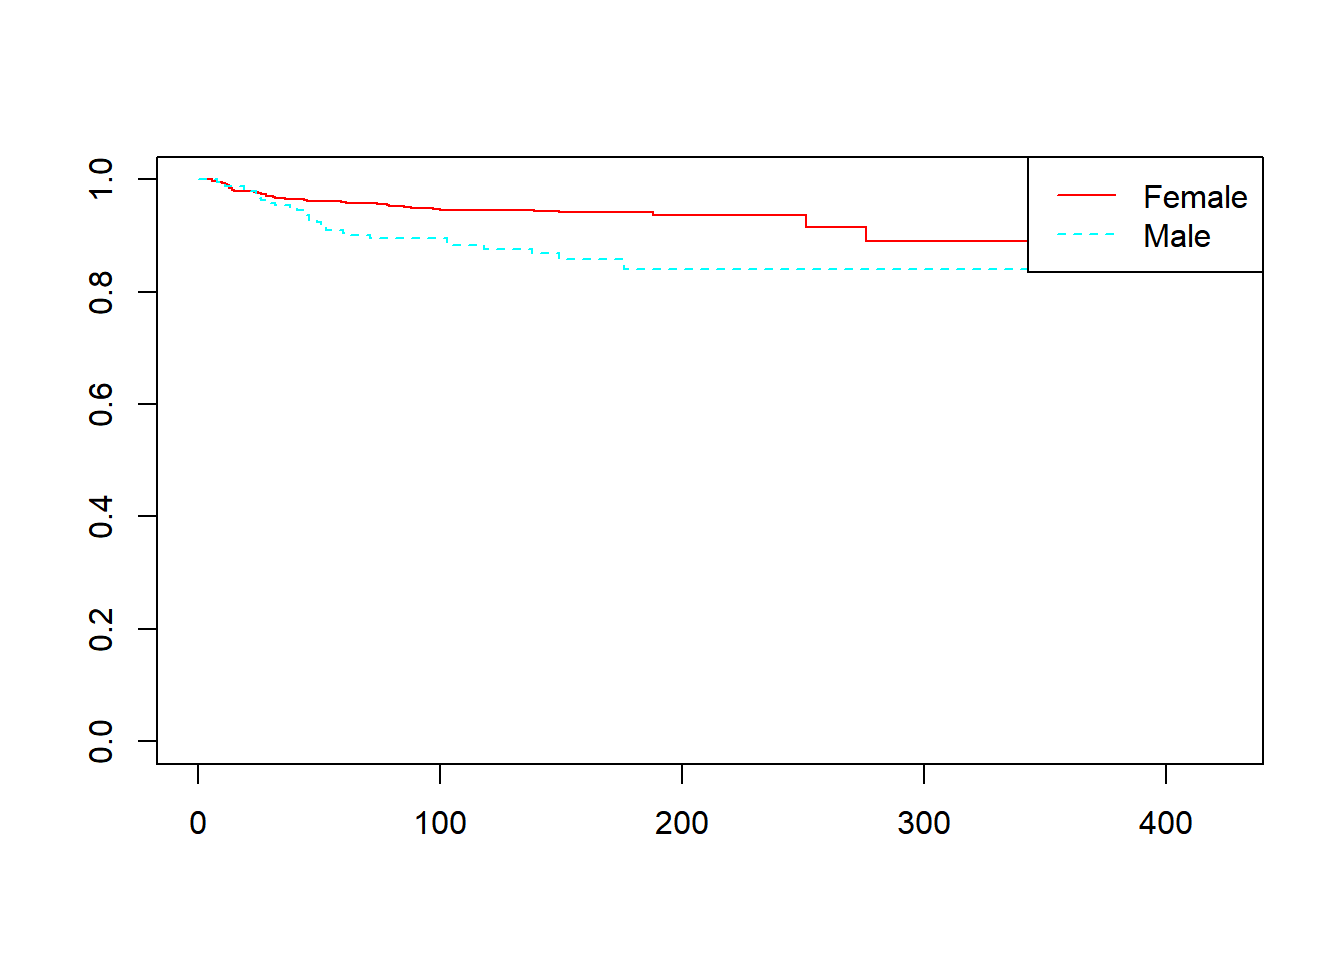
\includegraphics[keepaspectratio]{index_files/figure-pdf/plot_cox2-1.pdf}}

\subsubsection{ggsurvplot - risk.table
추가하기}\label{ggsurvplot---risk.table-uxcd94uxac00uxd558uxae30}

\begin{Shaded}
\begin{Highlighting}[]
\FunctionTok{library}\NormalTok{(survminer)}
\end{Highlighting}
\end{Shaded}

\begin{verbatim}
Loading required package: ggplot2
\end{verbatim}

\begin{verbatim}
Loading required package: ggpubr
\end{verbatim}

\begin{verbatim}

Attaching package: 'survminer'
\end{verbatim}

\begin{verbatim}
The following object is masked from 'package:survival':

    myeloma
\end{verbatim}

\begin{Shaded}
\begin{Highlighting}[]
\FunctionTok{ggsurvplot}\NormalTok{(}
\NormalTok{  km\_fit, }
  \AttributeTok{data =}\NormalTok{ rai\_recur,}
  \AttributeTok{conf.int =}\NormalTok{ T, }
  \AttributeTok{xscale =} \DecValTok{12}\NormalTok{, }\DocumentationTok{\#\# xscale can be "d\_y"}
  \AttributeTok{break.x.by =} \DecValTok{5}\SpecialCharTok{*}\DecValTok{12}\NormalTok{,}
  \AttributeTok{pval =}\NormalTok{ T, }
  \AttributeTok{pval.size =}\DecValTok{4}\NormalTok{, }
  \AttributeTok{surv.median.line =} \StringTok{"hv"}\NormalTok{,}
  \AttributeTok{risk.table =} \ConstantTok{TRUE}\NormalTok{, }\DocumentationTok{\#\# if TRUE, risk table is displayed under graph}
  \AttributeTok{legend.title=}\StringTok{"sex"}\NormalTok{, }
  \AttributeTok{legend.labs=}\FunctionTok{c}\NormalTok{(}\StringTok{"Female"}\NormalTok{,}\StringTok{"Male"}\NormalTok{),}
  \AttributeTok{palette =} \FunctionTok{c}\NormalTok{(}\StringTok{"\#E7B800"}\NormalTok{, }\StringTok{"\#2E9FDF"}\NormalTok{),}
\NormalTok{)}
\end{Highlighting}
\end{Shaded}

\begin{verbatim}
Warning in .add_surv_median(p, fit, type = surv.median.line, fun = fun, :
Median survival not reached.
\end{verbatim}

\pandocbounded{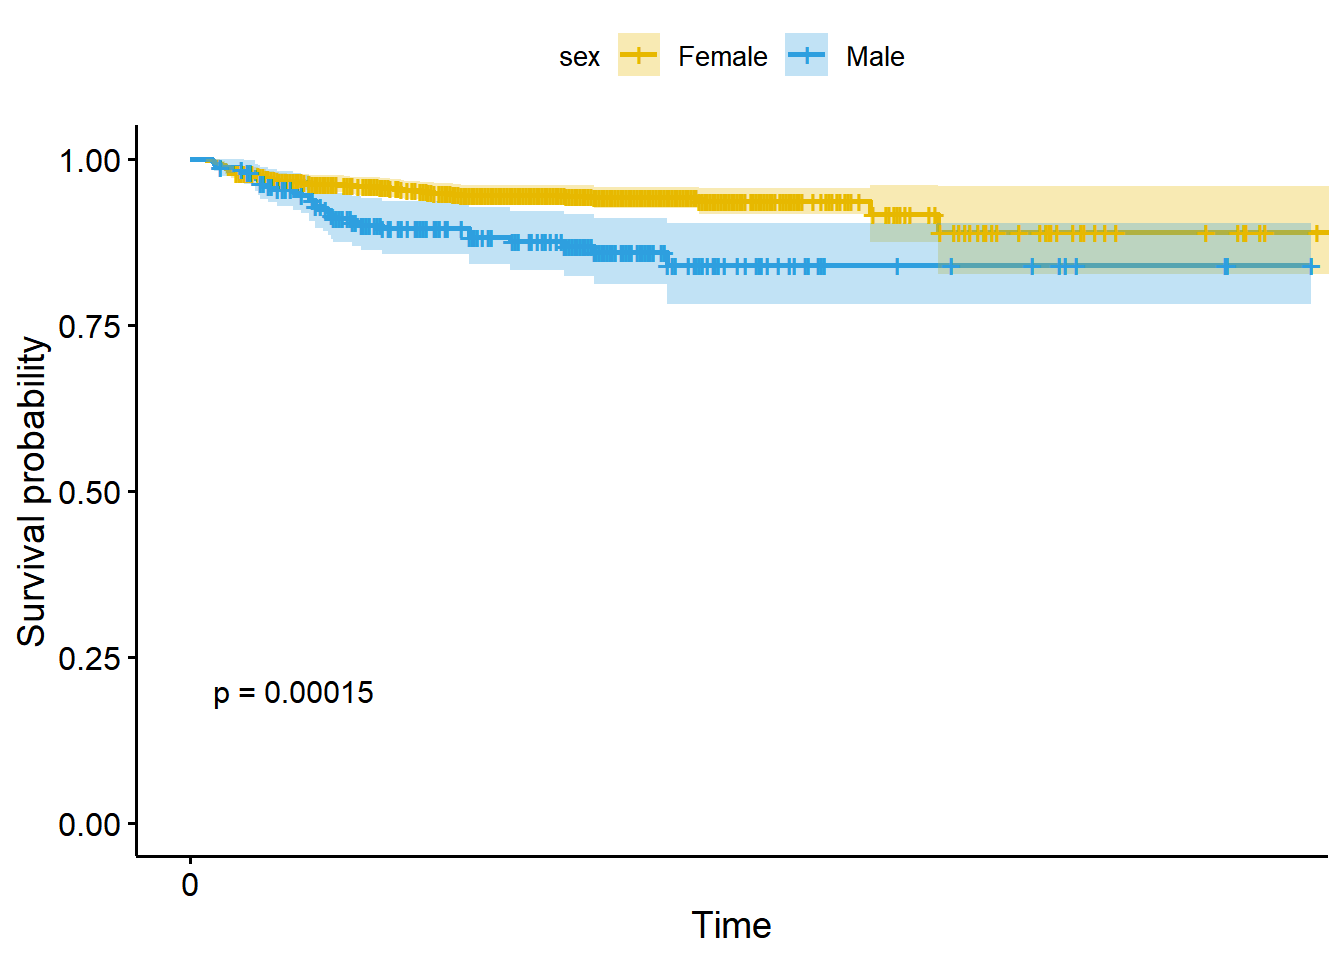
\includegraphics[keepaspectratio]{index_files/figure-pdf/ggsurvplot-1.pdf}}

\subsection{coxph}\label{coxph}

\subsubsection{cox 단변량}\label{cox-uxb2e8uxbcc0uxb7c9}

\[
h(t | X) = h_0(t) \exp(\beta_1 X_1 + \beta_2 X_2 + \dots + \beta_p X_p)
\] \#\#\#\# sex에 대한 단변량

\begin{Shaded}
\begin{Highlighting}[]
\NormalTok{univariate\_model }\OtherTok{\textless{}{-}} \FunctionTok{coxph}\NormalTok{(km }\SpecialCharTok{\textasciitilde{}}\NormalTok{ sex, }\AttributeTok{data =}\NormalTok{ rai\_recur)}
\FunctionTok{summary}\NormalTok{(univariate\_model)}
\end{Highlighting}
\end{Shaded}

\begin{verbatim}
Call:
coxph(formula = km ~ sex, data = rai_recur)

  n= 1180, number of events= 83 

       coef exp(coef) se(coef)     z Pr(>|z|)    
sexM 0.8430    2.3233   0.2287 3.686 0.000228 ***
---
Signif. codes:  0 '***' 0.001 '**' 0.01 '*' 0.05 '.' 0.1 ' ' 1

     exp(coef) exp(-coef) lower .95 upper .95
sexM     2.323     0.4304     1.484     3.637

Concordance= 0.58  (se = 0.027 )
Likelihood ratio test= 12.29  on 1 df,   p=5e-04
Wald test            = 13.59  on 1 df,   p=2e-04
Score (logrank) test = 14.41  on 1 df,   p=1e-04
\end{verbatim}

\paragraph{1️⃣ 검정 방법의
차이}\label{uxac80uxc815-uxbc29uxbc95uxc758-uxcc28uxc774}

\begin{itemize}
\tightlist
\item
  Likelihood Ratio Test: 모델 전체의 적합도를 평가하는 강력한 검정 방법.
\item
  Wald Test: 개별 회귀 계수가 0과 다른지 평가하지만, 샘플 크기가 작거나
  계수가 매우 크면 부정확할 수 있음.
\item
  Score Test: 작은 샘플에서도 안정적인 검정이지만, 일부 가정이 충족되지
  않으면 결과가 다를 수 있음.
\end{itemize}

\paragraph{2️⃣ 샘플 크기 및 데이터
특성}\label{uxc0d8uxd50c-uxd06cuxae30-uxbc0f-uxb370uxc774uxd130-uxd2b9uxc131}

\begin{itemize}
\tightlist
\item
  샘플 크기가 작을 때 → Wald Test는 불안정할 수 있음.
\item
  변수 간 다중공선성 → Wald Test와 LRT 결과가 다를 수 있음.
\item
  검열 데이터 비율이 높을 때 → Score Test가 다른 두 검정과 다를 수 있음.
\end{itemize}

\paragraph{\texorpdfstring{\textbf{📌 (1) Likelihood Ratio Test만
유의미하고 나머지는 유의미하지
않다면?}}{📌 (1) Likelihood Ratio Test만 유의미하고 나머지는 유의미하지 않다면?}}\label{likelihood-ratio-testuxb9cc-uxc720uxc758uxbbf8uxd558uxace0-uxb098uxba38uxc9c0uxb294-uxc720uxc758uxbbf8uxd558uxc9c0-uxc54auxb2e4uxba74}

\begin{itemize}
\tightlist
\item
  모델이 전체적으로는 의미가 있지만, 개별 변수의 효과가 강하지 않을 수
  있음.\\
\item
  Wald Test와 Score Test도 확인하면서 \textbf{개별 변수의 기여도를
  분석}해야 함.
\end{itemize}

\paragraph{\texorpdfstring{\textbf{📌 (2) Wald Test만
유의미하다면?}}{📌 (2) Wald Test만 유의미하다면?}}\label{wald-testuxb9cc-uxc720uxc758uxbbf8uxd558uxb2e4uxba74}

\begin{itemize}
\tightlist
\item
  특정 변수의 효과는 강하지만, 모델 전체가 데이터를 충분히 설명하지 못할
  수 있음.\\
\item
  변수 선택을 다시 검토하고 다중공선성을 점검해야 함.
\end{itemize}

\paragraph{\texorpdfstring{\textbf{📌 (3) Score Test만
유의미하다면?}}{📌 (3) Score Test만 유의미하다면?}}\label{score-testuxb9cc-uxc720uxc758uxbbf8uxd558uxb2e4uxba74}

\begin{itemize}
\tightlist
\item
  데이터가 잘 맞지만, 특정 변수의 효과가 불확실할 가능성이 있음.\\
\item
  모델의 구조와 데이터의 분포를 다시 확인해야 함.
\end{itemize}

\subsubsection{cox 단변량
반복}\label{cox-uxb2e8uxbcc0uxb7c9-uxbc18uxbcf5}

\begin{Shaded}
\begin{Highlighting}[]
\FunctionTok{mycph}\NormalTok{(}\FunctionTok{Surv}\NormalTok{(time, recur) }\SpecialCharTok{\textasciitilde{}}\NormalTok{ sex}\SpecialCharTok{+}\NormalTok{surgeon}\SpecialCharTok{+}\NormalTok{Risk}\SpecialCharTok{+}\NormalTok{pT}\SpecialCharTok{+}\NormalTok{gross\_ETE}\SpecialCharTok{+}\NormalTok{pN}\SpecialCharTok{+}\NormalTok{ENE, }\AttributeTok{data =}\NormalTok{ rai\_recur)}
\end{Highlighting}
\end{Shaded}

\begin{verbatim}

 mycph : perform coxph of individual expecting variables

 Call: Surv(time, recur) ~ sex + surgeon + Risk + pT + gross_ETE + pN +     ENE, data= rai_recur 
\end{verbatim}

\begin{verbatim}
                     HR   lcl    ucl     p
sexM               2.32  1.48   3.64 0.000
surgeonGS          8.87  0.92  85.71 0.059
surgeonKCCH        2.50  0.23  27.64 0.454
surgeonLBC         3.88  0.47  32.25 0.209
surgeonLGH         4.44  0.61  32.63 0.142
surgeonLMC         3.05  0.38  24.40 0.293
surgeonLYS        11.07  1.29  95.20 0.028
surgeonOKK        18.73  1.67 209.73 0.017
surgeonoutside    19.61  2.64 145.48 0.004
surgeonSYS         3.13  0.35  28.06 0.309
RiskIntermediate   0.39  0.25   0.62 0.000
RiskLow            0.08  0.03   0.19 0.000
pTT1b              2.65  1.37   5.12 0.004
pTT2               5.63  2.77  11.42 0.000
pTT3a              7.86  2.98  20.75 0.000
pTT3b              4.04  1.53  10.64 0.005
pTT4a             12.51  5.47  28.57 0.000
pTT4b            110.48 14.15 862.67 0.000
gross_ETEY         3.01  1.74   5.19 0.000
pNN1a              2.89  1.40   5.96 0.004
pNN1b              5.88  2.80  12.36 0.000
pNNx               1.92  0.58   6.34 0.285
ENEY               2.96  1.76   4.97 0.000
\end{verbatim}

\subsubsection{Multivariate Analysis}\label{multivariate-analysis}

\begin{Shaded}
\begin{Highlighting}[]
\NormalTok{cox\_model1 }\OtherTok{\textless{}{-}} \FunctionTok{coxph}\NormalTok{(}\FunctionTok{Surv}\NormalTok{(time, recur) }\SpecialCharTok{\textasciitilde{}}\NormalTok{ sex}\SpecialCharTok{+}\NormalTok{surgeon}\SpecialCharTok{+}\NormalTok{Risk}\SpecialCharTok{+}\NormalTok{pT}\SpecialCharTok{+}\NormalTok{gross\_ETE}\SpecialCharTok{+}\NormalTok{pN}\SpecialCharTok{+}\NormalTok{ENE, }\AttributeTok{data =}\NormalTok{ rai\_recur)}
\FunctionTok{summary}\NormalTok{(cox\_model1)}
\end{Highlighting}
\end{Shaded}

\begin{verbatim}
Call:
coxph(formula = Surv(time, recur) ~ sex + surgeon + Risk + pT + 
    gross_ETE + pN + ENE, data = rai_recur)

  n= 1180, number of events= 83 

                     coef exp(coef) se(coef)      z Pr(>|z|)   
sexM              0.45143   1.57055  0.25124  1.797  0.07237 . 
surgeonGS         1.82111   6.17873  1.17355  1.552  0.12071   
surgeonKCCH       0.84534   2.32877  1.23979  0.682  0.49534   
surgeonLBC        1.33518   3.80069  1.08259  1.233  0.21746   
surgeonLGH        1.39732   4.04434  1.02052  1.369  0.17093   
surgeonLMC        0.96762   2.63166  1.06429  0.909  0.36326   
surgeonLYS        2.35394  10.52698  1.12773  2.087  0.03686 * 
surgeonOKK        2.41672  11.20906  1.24459  1.942  0.05216 . 
surgeonoutside    2.53862  12.66221  1.02984  2.465  0.01370 * 
surgeonSYS        1.21122   3.35757  1.12605  1.076  0.28209   
RiskIntermediate -1.10109   0.33251  0.48798 -2.256  0.02404 * 
RiskLow          -1.94527   0.14295  0.69673 -2.792  0.00524 **
pTT1b             0.27864   1.32134  0.39790  0.700  0.48375   
pTT2              0.93086   2.53669  0.41840  2.225  0.02610 * 
pTT3a             1.33031   3.78220  0.56006  2.375  0.01753 * 
pTT3b            -0.01178   0.98829  0.78975 -0.015  0.98810   
pTT4a             0.68142   1.97669  0.73389  0.929  0.35315   
pTT4b             2.56213  12.96338  1.41329  1.813  0.06985 . 
gross_ETEY       -0.02956   0.97087  0.70231 -0.042  0.96643   
pNN1a             0.68781   1.98935  0.38041  1.808  0.07059 . 
pNN1b             0.87216   2.39207  0.41729  2.090  0.03661 * 
pNNx             -0.27631   0.75858  0.63063 -0.438  0.66128   
ENEY             -0.53707   0.58446  0.46306 -1.160  0.24612   
---
Signif. codes:  0 '***' 0.001 '**' 0.01 '*' 0.05 '.' 0.1 ' ' 1

                 exp(coef) exp(-coef) lower .95 upper .95
sexM                1.5706    0.63672   0.95983    2.5699
surgeonGS           6.1787    0.16185   0.61940   61.6354
surgeonKCCH         2.3288    0.42941   0.20503   26.4507
surgeonLBC          3.8007    0.26311   0.45537   31.7224
surgeonLGH          4.0443    0.24726   0.54724   29.8895
surgeonLMC          2.6317    0.37999   0.32682   21.1911
surgeonLYS         10.5270    0.09499   1.15445   95.9916
surgeonOKK         11.2091    0.08921   0.97762  128.5198
surgeonoutside     12.6622    0.07898   1.68232   95.3038
surgeonSYS          3.3576    0.29783   0.36943   30.5153
RiskIntermediate    0.3325    3.00745   0.12777    0.8653
RiskLow             0.1429    6.99550   0.03649    0.5601
pTT1b               1.3213    0.75681   0.60578    2.8821
pTT2                2.5367    0.39422   1.11717    5.7599
pTT3a               3.7822    0.26440   1.26190   11.3361
pTT3b               0.9883    1.01185   0.21021    4.6465
pTT4a               1.9767    0.50590   0.46908    8.3297
pTT4b              12.9634    0.07714   0.81232  206.8754
gross_ETEY          0.9709    1.03000   0.24511    3.8457
pNN1a               1.9894    0.50268   0.94386    4.1929
pNN1b               2.3921    0.41805   1.05579    5.4196
pNNx                0.7586    1.31826   0.22040    2.6109
ENEY                0.5845    1.71098   0.23583    1.4485

Concordance= 0.792  (se = 0.024 )
Likelihood ratio test= 112.5  on 23 df,   p=9e-14
Wald test            = 110.8  on 23 df,   p=2e-13
Score (logrank) test = 176.7  on 23 df,   p=<2e-16
\end{verbatim}

\subsubsection{Multivariate - anova}\label{multivariate---anova}

\begin{itemize}
\tightlist
\item
  anova(cox\_model1)는 Cox 회귀 모델에서 각 변수의 기여도를 평가하는
  역할을 함.
\item
  각 변수가 모델에 얼마나 중요한지 평가하고, p-value를 기반으로 불필요한
  변수를 제거할 수 있음.
\item
  Deviance 값이 크고 p-value가 낮은 변수는 중요한 변수이며, p-value가
  높으면 제거를 고려할 수 있음.
\end{itemize}

\begin{Shaded}
\begin{Highlighting}[]
\FunctionTok{anova}\NormalTok{(cox\_model1)}
\end{Highlighting}
\end{Shaded}

\begin{verbatim}
Analysis of Deviance Table
 Cox model: response is Surv(time, recur)
Terms added sequentially (first to last)

           loglik   Chisq Df Pr(>|Chi|)    
NULL      -567.06                          
sex       -560.92 12.2949  1  0.0004542 ***
surgeon   -540.38 41.0665  9  4.864e-06 ***
Risk      -521.33 38.1136  2  5.293e-09 ***
pT        -515.05 12.5592  6  0.0505954 .  
gross_ETE -515.03  0.0306  1  0.8610979    
pN        -511.51  7.0409  3  0.0706054 .  
ENE       -510.84  1.3484  1  0.2455630    
---
Signif. codes:  0 '***' 0.001 '**' 0.01 '*' 0.05 '.' 0.1 ' ' 1
\end{verbatim}

\begin{itemize}
\tightlist
\item
  Cox 회귀 모델에서는 로그 우도를 최대화(즉, 덜 음수로 만듦) 하는
  방향으로 최적화를 수행

  \begin{itemize}
  \tightlist
  \item
    NULL 모델 (loglik = -567.06) → 변수가 없는 기본 모델
  \item
    모델이 점점 좋아질수록 loglik 값 증가
  \item
    sex 추가 후: loglik = -560.92 (증가)
  \item
    surgeon 추가 후: loglik = -540.38 (더 증가)
  \item
    Risk 추가 후: loglik = -521.33 (더 증가)
  \end{itemize}
\end{itemize}

\subsubsection{Multivariate - refit}\label{multivariate---refit}

\begin{Shaded}
\begin{Highlighting}[]
\NormalTok{cox\_model\_refit }\OtherTok{\textless{}{-}} \FunctionTok{coxph}\NormalTok{(}\FunctionTok{Surv}\NormalTok{(time, recur) }\SpecialCharTok{\textasciitilde{}}\NormalTok{ sex}\SpecialCharTok{+}\NormalTok{surgeon}\SpecialCharTok{+}\NormalTok{Risk, }\AttributeTok{data =}\NormalTok{ rai\_recur)}
\FunctionTok{summary}\NormalTok{(cox\_model\_refit)}
\end{Highlighting}
\end{Shaded}

\begin{verbatim}
Call:
coxph(formula = Surv(time, recur) ~ sex + surgeon + Risk, data = rai_recur)

  n= 1180, number of events= 83 

                    coef exp(coef) se(coef)      z Pr(>|z|)    
sexM              0.4982    1.6457   0.2395  2.080 0.037565 *  
surgeonGS         2.1328    8.4382   1.1591  1.840 0.065765 .  
surgeonKCCH       1.0549    2.8717   1.2288  0.859 0.390615    
surgeonLBC        1.4876    4.4264   1.0806  1.377 0.168610    
surgeonLGH        1.4732    4.3630   1.0184  1.447 0.148017    
surgeonLMC        1.0942    2.9867   1.0618  1.030 0.302797    
surgeonLYS        2.4262   11.3163   1.0983  2.209 0.027169 *  
surgeonOKK        2.7836   16.1772   1.2349  2.254 0.024193 *  
surgeonoutside    2.7641   15.8650   1.0244  2.698 0.006967 ** 
surgeonSYS        1.3356    3.8024   1.1204  1.192 0.233240    
RiskIntermediate -0.9051    0.4045   0.2375 -3.811 0.000139 ***
RiskLow          -2.2999    0.1003   0.4506 -5.105 3.31e-07 ***
---
Signif. codes:  0 '***' 0.001 '**' 0.01 '*' 0.05 '.' 0.1 ' ' 1

                 exp(coef) exp(-coef) lower .95 upper .95
sexM                1.6457    0.60765   1.02906    2.6318
surgeonGS           8.4382    0.11851   0.87021   81.8234
surgeonKCCH         2.8717    0.34822   0.25835   31.9211
surgeonLBC          4.4264    0.22592   0.53245   36.7971
surgeonLGH          4.3630    0.22920   0.59284   32.1094
surgeonLMC          2.9867    0.33482   0.37270   23.9346
surgeonLYS         11.3163    0.08837   1.31470   97.4044
surgeonOKK         16.1772    0.06182   1.43790  182.0038
surgeonoutside     15.8650    0.06303   2.13064  118.1329
surgeonSYS          3.8024    0.26299   0.42299   34.1799
RiskIntermediate    0.4045    2.47207   0.25397    0.6443
RiskLow             0.1003    9.97356   0.04146    0.2425

Concordance= 0.761  (se = 0.025 )
Likelihood ratio test= 91.47  on 12 df,   p=3e-14
Wald test            = 86.44  on 12 df,   p=2e-13
Score (logrank) test = 114.2  on 12 df,   p=<2e-16
\end{verbatim}

\subsubsection{survfit plot}\label{survfit-plot}

\begin{Shaded}
\begin{Highlighting}[]
\FunctionTok{plot}\NormalTok{(}\FunctionTok{survfit}\NormalTok{(cox\_model1), }\AttributeTok{ylim =} \FunctionTok{c}\NormalTok{(}\FloatTok{0.6}\NormalTok{,}\DecValTok{1}\NormalTok{),}\AttributeTok{xlab =} \StringTok{"months"}\NormalTok{,}
\AttributeTok{ylab =} \StringTok{"Proportion not reached"}\NormalTok{)}
\end{Highlighting}
\end{Shaded}

\pandocbounded{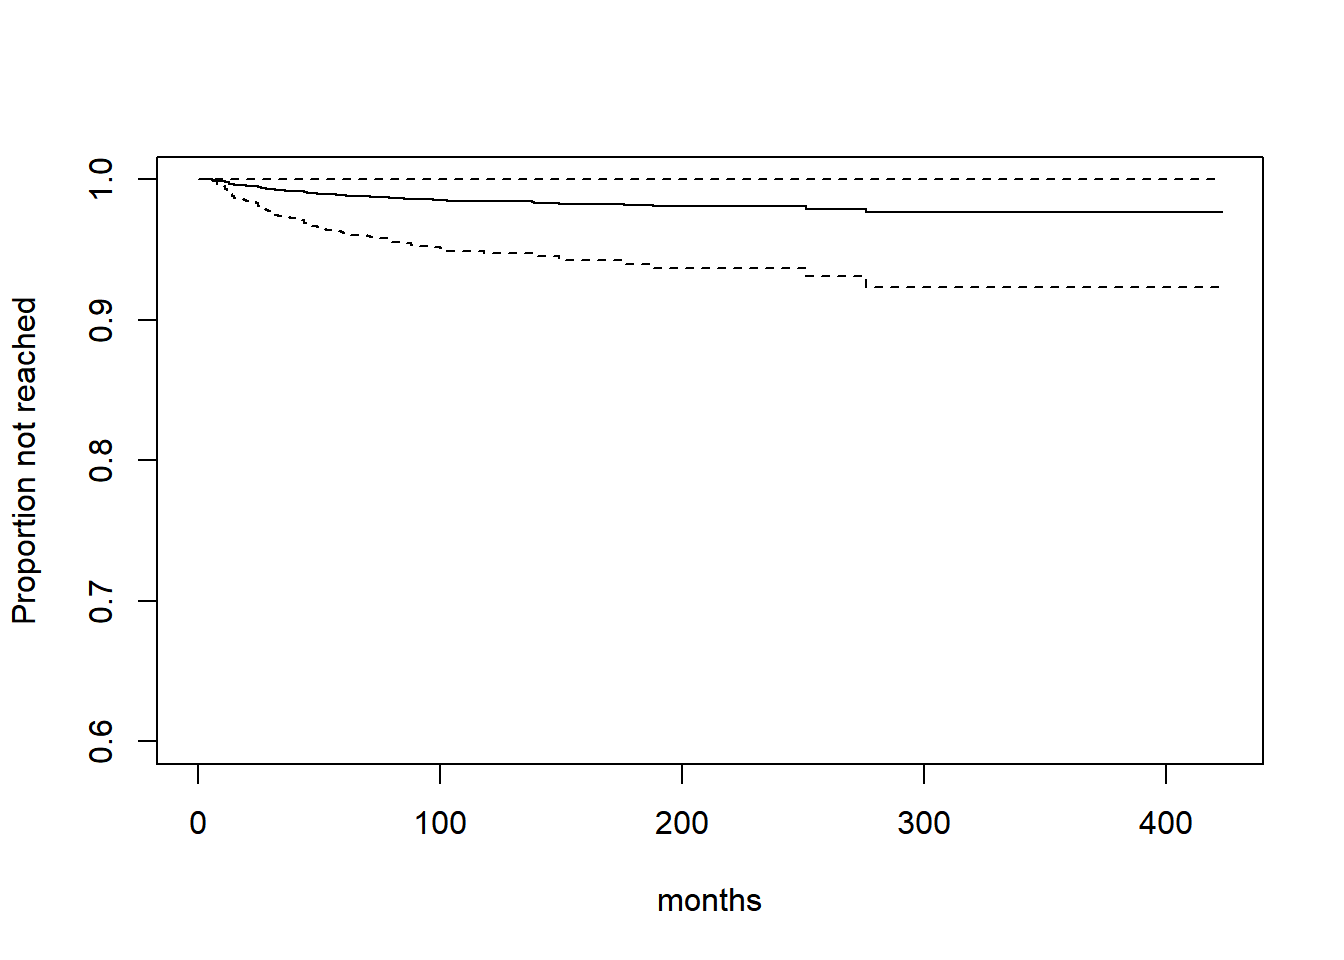
\includegraphics[keepaspectratio]{index_files/figure-pdf/plot3-1.pdf}}

\subsection{잔차분석}\label{uxc794uxcc28uxbd84uxc11d}

\subsubsection{time histogram}\label{time-histogram}

\begin{Shaded}
\begin{Highlighting}[]
\FunctionTok{with}\NormalTok{(rai\_recur, }\FunctionTok{hist}\NormalTok{(time}\SpecialCharTok{/}\DecValTok{12}\NormalTok{, }\AttributeTok{breaks =} \DecValTok{40}\NormalTok{, }\AttributeTok{main =} \StringTok{"Histogram of time"}\NormalTok{))}
\end{Highlighting}
\end{Shaded}

\pandocbounded{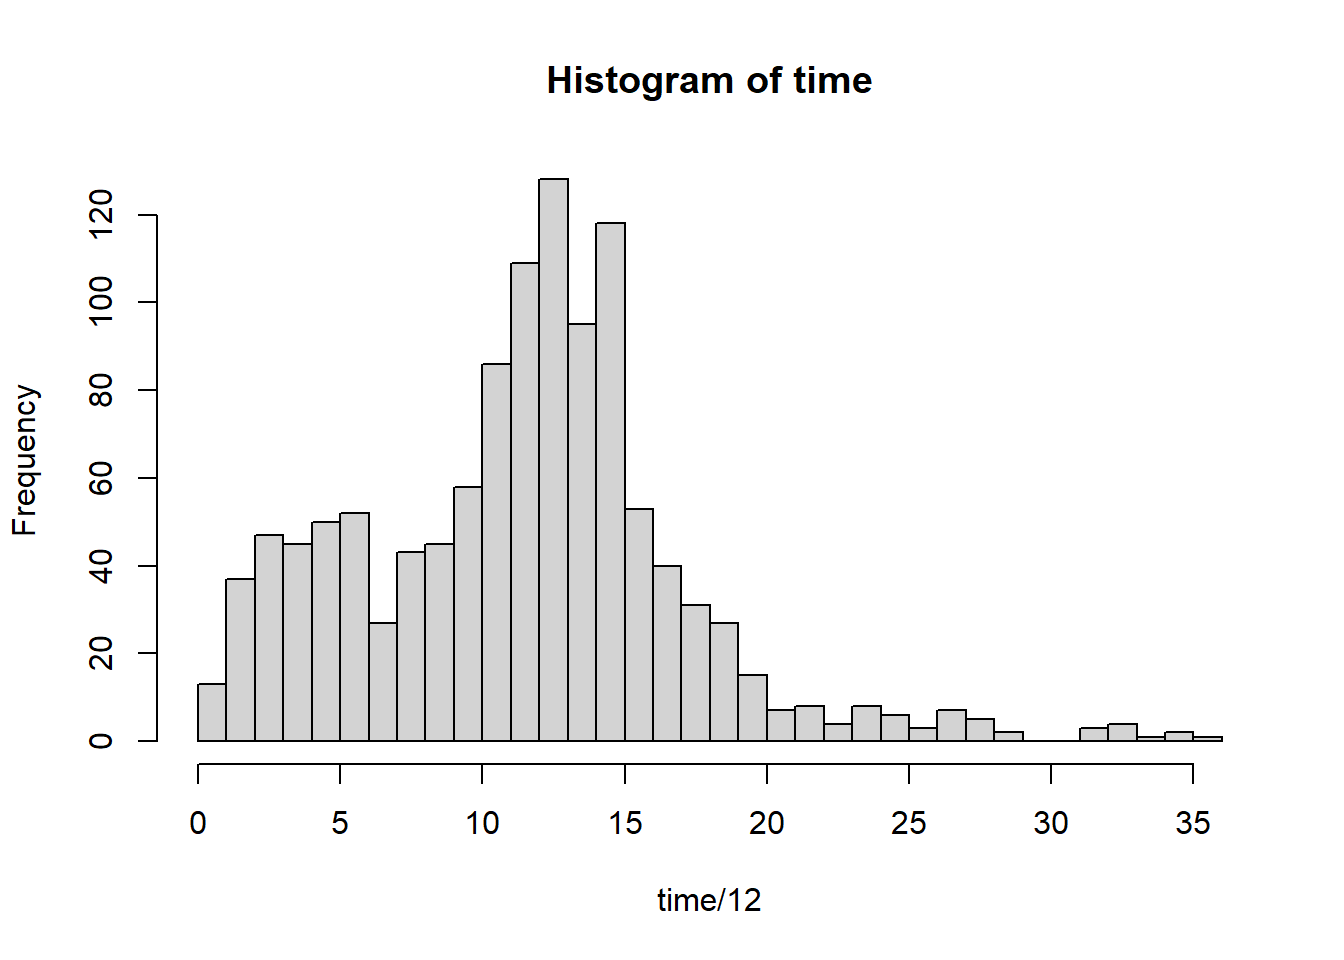
\includegraphics[keepaspectratio]{index_files/figure-pdf/time_hist-1.pdf}}

\subsubsection{age histogram}\label{age-histogram}

\begin{Shaded}
\begin{Highlighting}[]
\FunctionTok{with}\NormalTok{(rai\_recur, }\FunctionTok{hist}\NormalTok{(age, }\AttributeTok{breaks =} \DecValTok{16}\NormalTok{, }\AttributeTok{main =} \StringTok{"Histogram of age"}\NormalTok{))}
\end{Highlighting}
\end{Shaded}

\pandocbounded{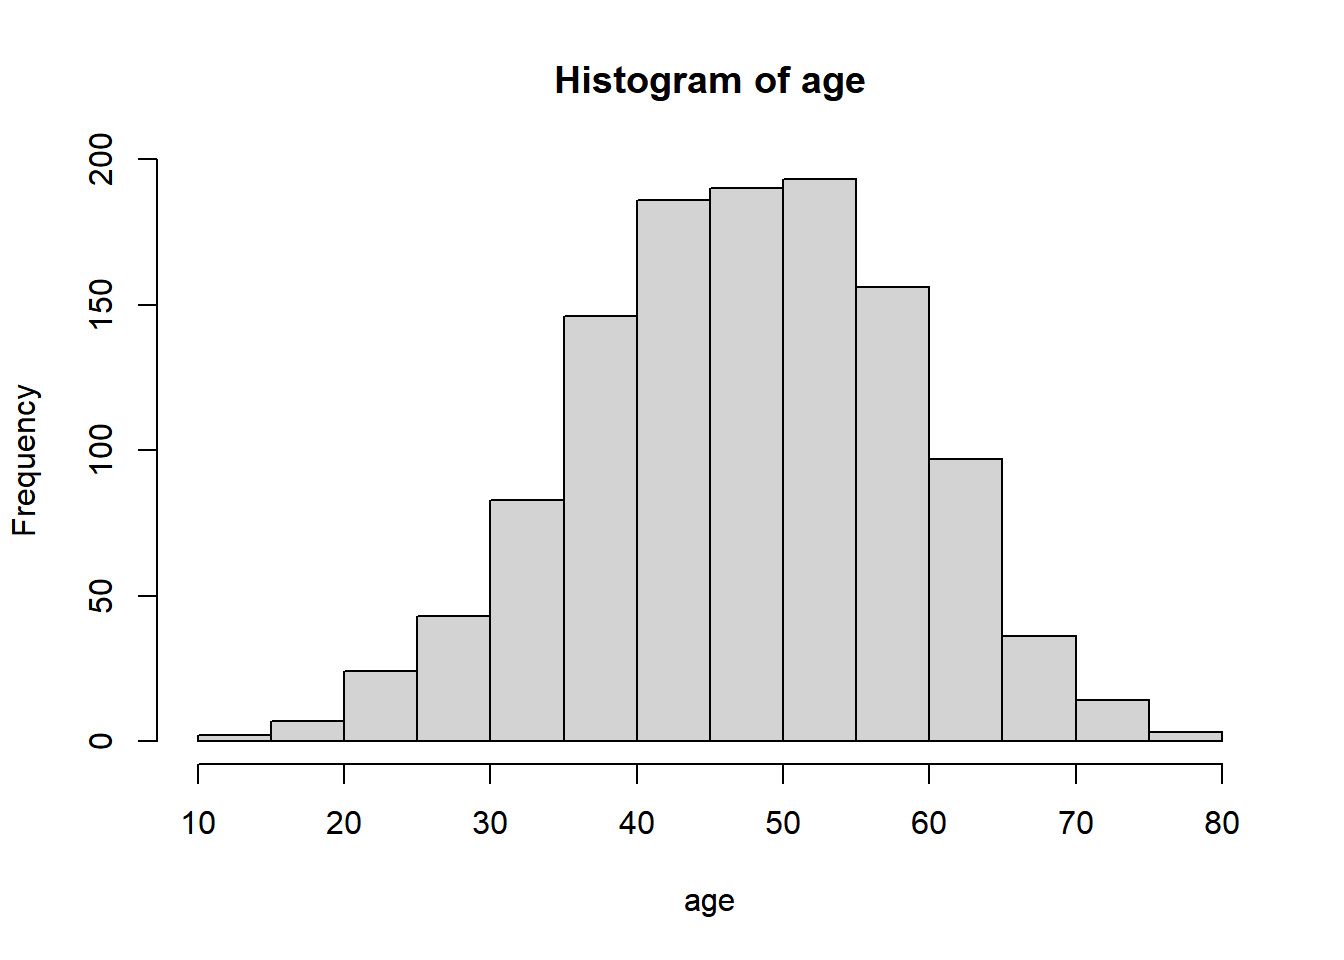
\includegraphics[keepaspectratio]{index_files/figure-pdf/age_hist-1.pdf}}

\subsubsection{size histogram}\label{size-histogram}

\begin{Shaded}
\begin{Highlighting}[]
\FunctionTok{with}\NormalTok{(rai\_recur, }\FunctionTok{hist}\NormalTok{(size, }\AttributeTok{breaks =} \DecValTok{16}\NormalTok{, }\AttributeTok{main =} \StringTok{"Histogram of age"}\NormalTok{))}
\end{Highlighting}
\end{Shaded}

\pandocbounded{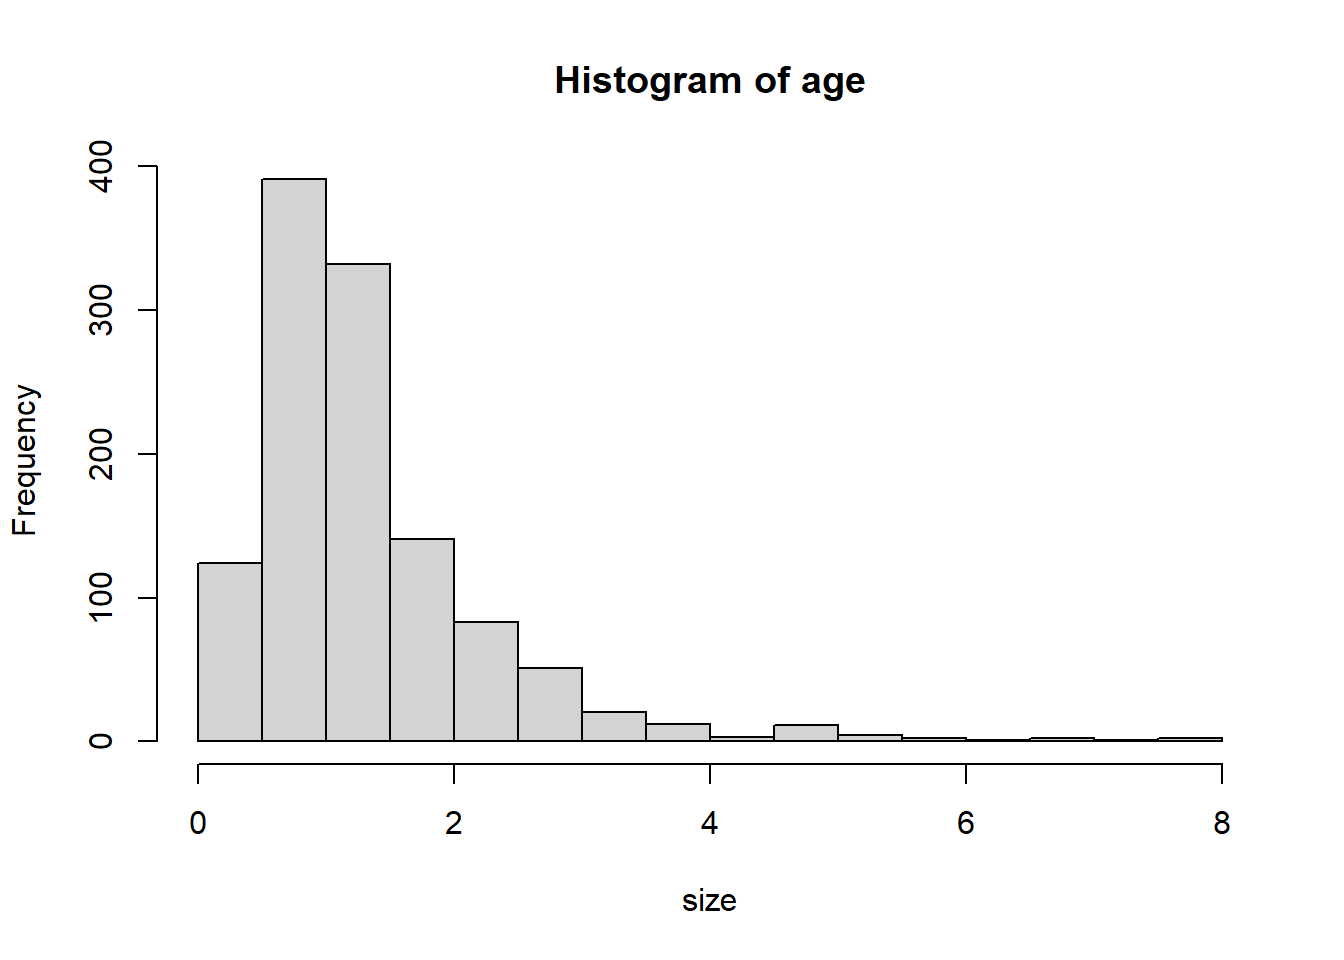
\includegraphics[keepaspectratio]{index_files/figure-pdf/size_hist-1.pdf}}

\subsubsection{age residual}\label{age-residual}

\begin{Shaded}
\begin{Highlighting}[]
\NormalTok{m1 }\OtherTok{\textless{}{-}} \FunctionTok{coxph}\NormalTok{(}\FunctionTok{Surv}\NormalTok{(time,recur)}\SpecialCharTok{\textasciitilde{}}\DecValTok{1}\NormalTok{,}\AttributeTok{data =}\NormalTok{ rai\_recur)}
\NormalTok{rai\_recur}\SpecialCharTok{$}\NormalTok{resid }\OtherTok{\textless{}{-}} \FunctionTok{residuals}\NormalTok{(m1, }\AttributeTok{type =} \StringTok{"martingale"}\NormalTok{)}
\NormalTok{rai\_recur }\SpecialCharTok{\%\textgreater{}\%} \FunctionTok{ggplot}\NormalTok{(}\FunctionTok{aes}\NormalTok{(age,resid))}\SpecialCharTok{+}\FunctionTok{geom\_point}\NormalTok{()}\SpecialCharTok{+}\FunctionTok{geom\_smooth}\NormalTok{()}\SpecialCharTok{+}\FunctionTok{theme\_classic}\NormalTok{()}
\end{Highlighting}
\end{Shaded}

\begin{verbatim}
`geom_smooth()` using method = 'gam' and formula = 'y ~ s(x, bs = "cs")'
\end{verbatim}

\pandocbounded{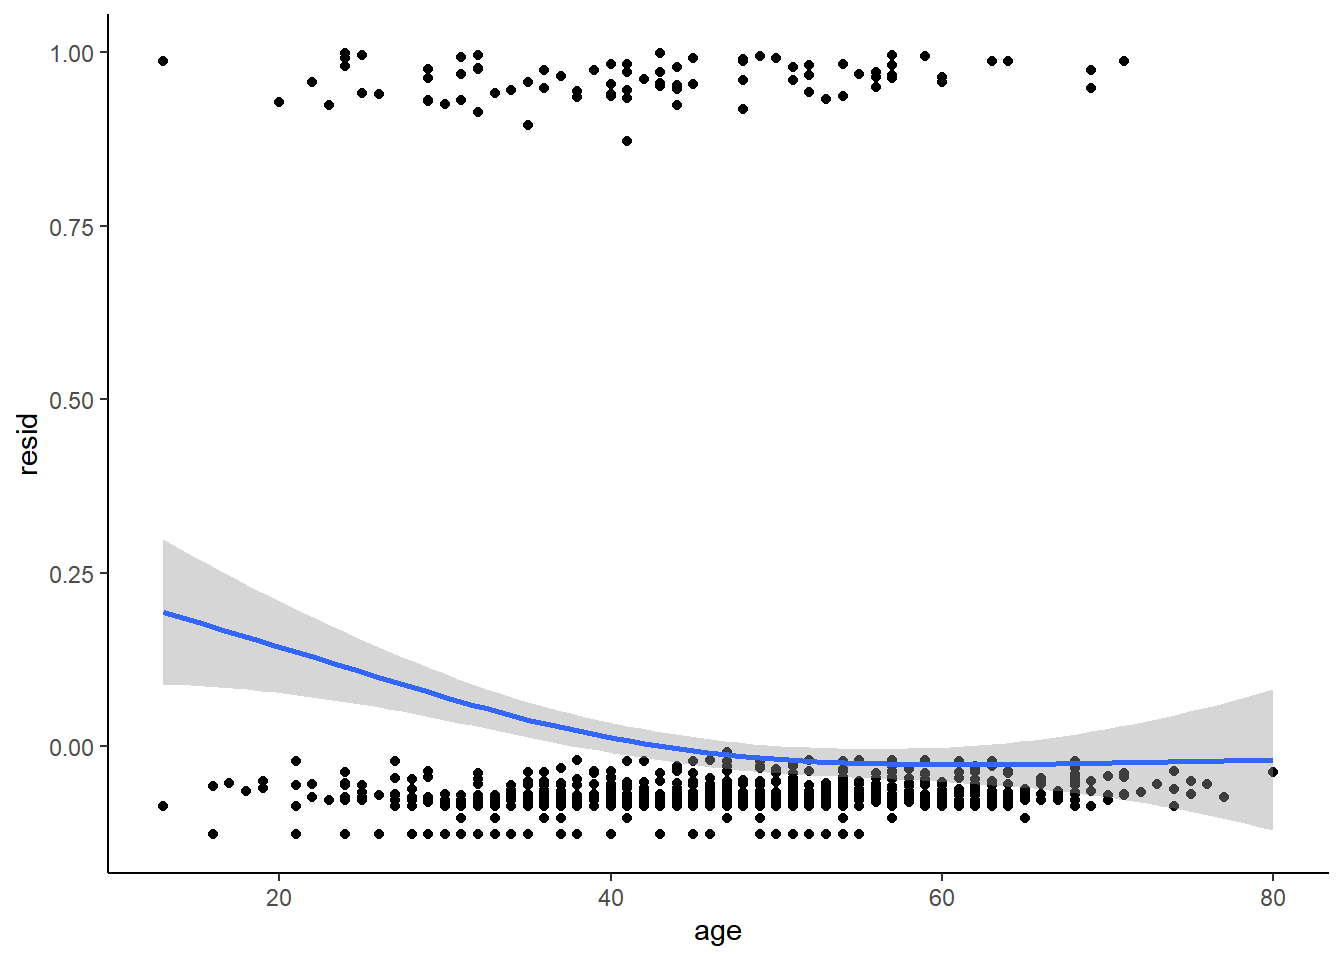
\includegraphics[keepaspectratio]{index_files/figure-pdf/age_residual-1.pdf}}

\subsubsection{size residual}\label{size-residual}

\begin{Shaded}
\begin{Highlighting}[]
\NormalTok{rai\_recur }\SpecialCharTok{\%\textgreater{}\%} \FunctionTok{ggplot}\NormalTok{(}\FunctionTok{aes}\NormalTok{(size,resid))}\SpecialCharTok{+}\FunctionTok{geom\_point}\NormalTok{()}\SpecialCharTok{+}\FunctionTok{geom\_smooth}\NormalTok{()}\SpecialCharTok{+}\FunctionTok{theme\_classic}\NormalTok{()}
\end{Highlighting}
\end{Shaded}

\begin{verbatim}
`geom_smooth()` using method = 'gam' and formula = 'y ~ s(x, bs = "cs")'
\end{verbatim}

\pandocbounded{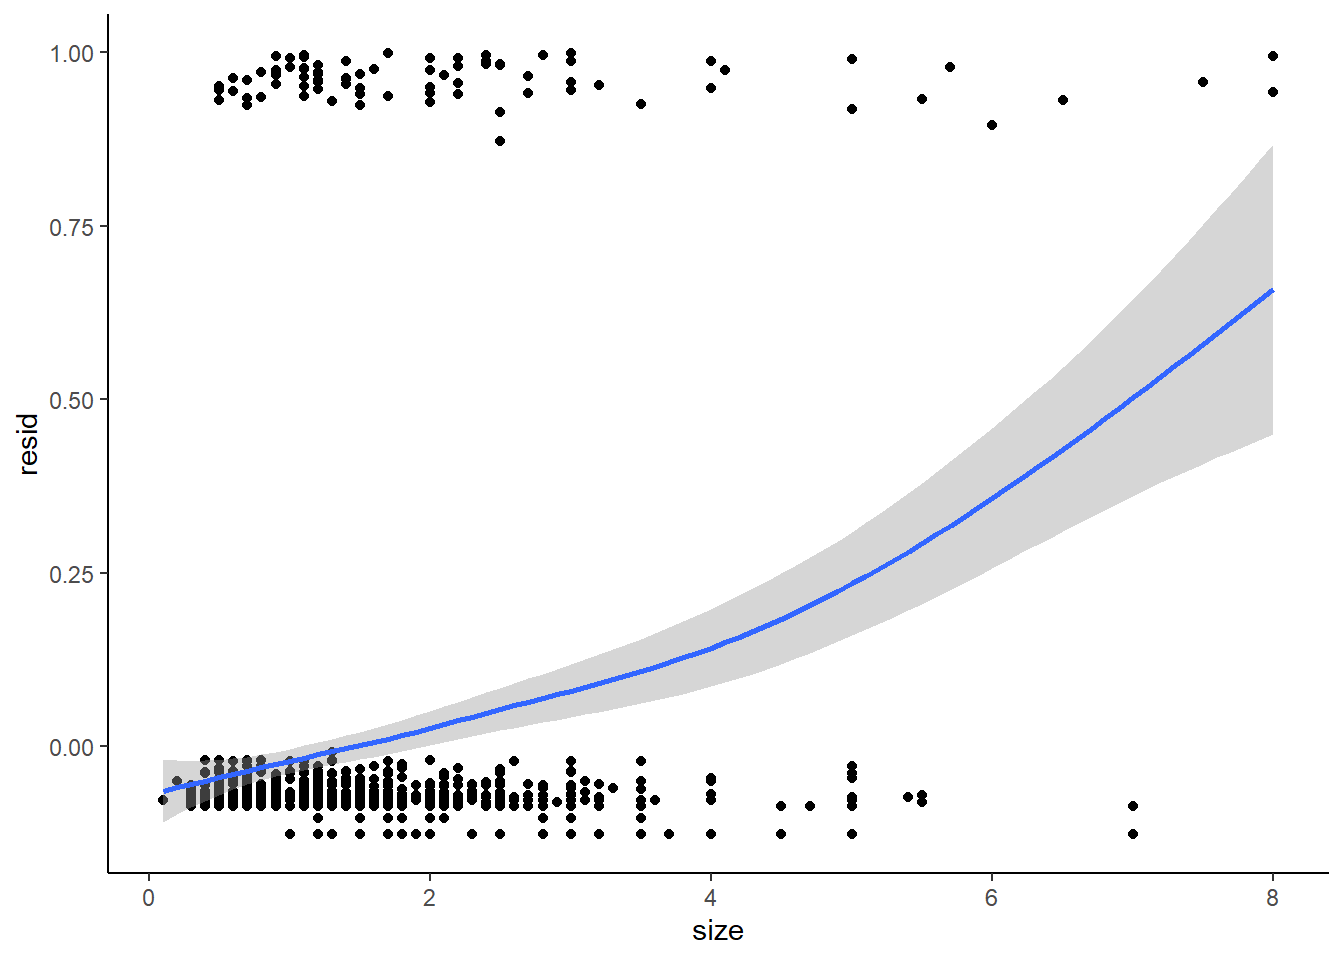
\includegraphics[keepaspectratio]{index_files/figure-pdf/size_residual-1.pdf}}

\subsection{연속형변수와
cox}\label{uxc5f0uxc18duxd615uxbcc0uxc218uxc640-cox}

\subsubsection{cox 단변량
반복2}\label{cox-uxb2e8uxbcc0uxb7c9-uxbc18uxbcf52}

\begin{Shaded}
\begin{Highlighting}[]
\FunctionTok{mycph}\NormalTok{(}\FunctionTok{Surv}\NormalTok{(time, recur) }\SpecialCharTok{\textasciitilde{}}\NormalTok{ age}\SpecialCharTok{+}\NormalTok{sex}\SpecialCharTok{+}\NormalTok{surgeon}\SpecialCharTok{+}\NormalTok{Risk}\SpecialCharTok{+}\NormalTok{pT}\SpecialCharTok{+}\NormalTok{size}\SpecialCharTok{+}\NormalTok{gross\_ETE}\SpecialCharTok{+}\NormalTok{pN}\SpecialCharTok{+}\NormalTok{ENE, }\AttributeTok{data =}\NormalTok{ rai\_recur)}
\end{Highlighting}
\end{Shaded}

\begin{verbatim}

 mycph : perform coxph of individual expecting variables

 Call: Surv(time, recur) ~ age + sex + surgeon + Risk + pT + size +     gross_ETE + pN + ENE, data= rai_recur 
\end{verbatim}

\begin{verbatim}
                     HR   lcl    ucl     p
age                0.96  0.94   0.98 0.000
sexM               2.32  1.48   3.64 0.000
surgeonGS          8.87  0.92  85.71 0.059
surgeonKCCH        2.50  0.23  27.64 0.454
surgeonLBC         3.88  0.47  32.25 0.209
surgeonLGH         4.44  0.61  32.63 0.142
surgeonLMC         3.05  0.38  24.40 0.293
surgeonLYS        11.07  1.29  95.20 0.028
surgeonOKK        18.73  1.67 209.73 0.017
surgeonoutside    19.61  2.64 145.48 0.004
surgeonSYS         3.13  0.35  28.06 0.309
RiskIntermediate   0.39  0.25   0.62 0.000
RiskLow            0.08  0.03   0.19 0.000
pTT1b              2.65  1.37   5.12 0.004
pTT2               5.63  2.77  11.42 0.000
pTT3a              7.86  2.98  20.75 0.000
pTT3b              4.04  1.53  10.64 0.005
pTT4a             12.51  5.47  28.57 0.000
pTT4b            110.48 14.15 862.67 0.000
size               1.61  1.43   1.81 0.000
gross_ETEY         3.01  1.74   5.19 0.000
pNN1a              2.89  1.40   5.96 0.004
pNN1b              5.88  2.80  12.36 0.000
pNNx               1.92  0.58   6.34 0.285
ENEY               2.96  1.76   4.97 0.000
\end{verbatim}

\subsubsection{Multivariate Analysis 2}\label{multivariate-analysis-2}

\begin{Shaded}
\begin{Highlighting}[]
\NormalTok{cox\_model2 }\OtherTok{\textless{}{-}} \FunctionTok{coxph}\NormalTok{(}\FunctionTok{Surv}\NormalTok{(time, recur) }\SpecialCharTok{\textasciitilde{}}\NormalTok{ age}\SpecialCharTok{+}\NormalTok{sex}\SpecialCharTok{+}\NormalTok{surgeon}\SpecialCharTok{+}\NormalTok{Risk}\SpecialCharTok{+}\NormalTok{pT}\SpecialCharTok{+}\NormalTok{size}\SpecialCharTok{+}\NormalTok{gross\_ETE}\SpecialCharTok{+}\NormalTok{pN}\SpecialCharTok{+}\NormalTok{ENE, }\AttributeTok{data =}\NormalTok{ rai\_recur)}
\FunctionTok{summary}\NormalTok{(cox\_model2)}
\end{Highlighting}
\end{Shaded}

\begin{verbatim}
Call:
coxph(formula = Surv(time, recur) ~ age + sex + surgeon + Risk + 
    pT + size + gross_ETE + pN + ENE, data = rai_recur)

  n= 1180, number of events= 83 

                      coef exp(coef)  se(coef)      z Pr(>|z|)   
age              -0.014008  0.986090  0.009941 -1.409  0.15880   
sexM              0.328854  1.389375  0.258244  1.273  0.20287   
surgeonGS         1.671413  5.319680  1.179586  1.417  0.15650   
surgeonKCCH       1.142594  3.134888  1.247675  0.916  0.35978   
surgeonLBC        1.494638  4.457724  1.085987  1.376  0.16873   
surgeonLGH        1.553412  4.727573  1.024719  1.516  0.12953   
surgeonLMC        1.203669  3.332322  1.068352  1.127  0.25989   
surgeonLYS        2.388710 10.899427  1.131419  2.111  0.03475 * 
surgeonOKK        2.472220 11.848726  1.248650  1.980  0.04771 * 
surgeonoutside    2.607921 13.570810  1.031837  2.527  0.01149 * 
surgeonSYS        1.392094  4.023265  1.130279  1.232  0.21808   
RiskIntermediate -1.097029  0.333862  0.461238 -2.378  0.01739 * 
RiskLow          -1.946380  0.142790  0.676862 -2.876  0.00403 **
pTT1b            -0.011762  0.988307  0.407939 -0.029  0.97700   
pTT2              0.151581  1.163673  0.485457  0.312  0.75485   
pTT3a            -0.302922  0.738657  0.805684 -0.376  0.70693   
pTT3b            -0.772746  0.461743  0.853145 -0.906  0.36506   
pTT4a            -0.260828  0.770414  0.792535 -0.329  0.74208   
pTT4b             1.765631  5.845260  1.428885  1.236  0.21658   
size              0.380317  1.462748  0.123769  3.073  0.00212 **
gross_ETEY        0.317829  1.374141  0.687014  0.463  0.64363   
pNN1a             0.671573  1.957313  0.384123  1.748  0.08041 . 
pNN1b             0.778179  2.177504  0.421857  1.845  0.06509 . 
pNNx             -0.633082  0.530953  0.648227 -0.977  0.32875   
ENEY             -0.526398  0.590729  0.448249 -1.174  0.24026   
---
Signif. codes:  0 '***' 0.001 '**' 0.01 '*' 0.05 '.' 0.1 ' ' 1

                 exp(coef) exp(-coef) lower .95 upper .95
age                 0.9861    1.01411   0.96706    1.0055
sexM                1.3894    0.71975   0.83753    2.3048
surgeonGS           5.3197    0.18798   0.52701   53.6972
surgeonKCCH         3.1349    0.31899   0.27177   36.1614
surgeonLBC          4.4577    0.22433   0.53054   37.4547
surgeonLGH          4.7276    0.21153   0.63445   35.2274
surgeonLMC          3.3323    0.30009   0.41055   27.0477
surgeonLYS         10.8994    0.09175   1.18669  100.1081
surgeonOKK         11.8487    0.08440   1.02522  136.9381
surgeonoutside     13.5708    0.07369   1.79599  102.5433
surgeonSYS          4.0233    0.24855   0.43902   36.8700
RiskIntermediate    0.3339    2.99525   0.13519    0.8245
RiskLow             0.1428    7.00329   0.03789    0.5381
pTT1b               0.9883    1.01183   0.44428    2.1985
pTT2                1.1637    0.85935   0.44938    3.0134
pTT3a               0.7387    1.35381   0.15228    3.5830
pTT3b               0.4617    2.16571   0.08674    2.4581
pTT4a               0.7704    1.29800   0.16297    3.6419
pTT4b               5.8453    0.17108   0.35525   96.1773
size                1.4627    0.68364   1.14767    1.8643
gross_ETEY          1.3741    0.72773   0.35747    5.2823
pNN1a               1.9573    0.51090   0.92192    4.1555
pNN1b               2.1775    0.45924   0.95252    4.9779
pNNx                0.5310    1.88341   0.14903    1.8916
ENEY                0.5907    1.69282   0.24538    1.4221

Concordance= 0.8  (se = 0.025 )
Likelihood ratio test= 123.5  on 25 df,   p=5e-15
Wald test            = 128  on 25 df,   p=9e-16
Score (logrank) test = 201.3  on 25 df,   p=<2e-16
\end{verbatim}

\subsubsection{Multivariate - anova 2}\label{multivariate---anova-2}

\begin{Shaded}
\begin{Highlighting}[]
\FunctionTok{anova}\NormalTok{(cox\_model2)}
\end{Highlighting}
\end{Shaded}

\begin{verbatim}
Analysis of Deviance Table
 Cox model: response is Surv(time, recur)
Terms added sequentially (first to last)

           loglik   Chisq Df Pr(>|Chi|)    
NULL      -567.06                          
age       -558.29 17.5547  1  2.792e-05 ***
sex       -553.89  8.7974  1   0.003017 ** 
surgeon   -536.85 34.0796  9  8.650e-05 ***
Risk      -518.67 36.3495  2  1.279e-08 ***
pT        -513.09 11.1599  6   0.083560 .  
size      -510.44  5.2994  1   0.021333 *  
gross_ETE -510.27  0.3462  1   0.556248    
pN        -505.99  8.5666  3   0.035645 *  
ENE       -505.30  1.3668  1   0.242362    
---
Signif. codes:  0 '***' 0.001 '**' 0.01 '*' 0.05 '.' 0.1 ' ' 1
\end{verbatim}

\subsubsection{Multivariate refit 2}\label{multivariate-refit-2}

\begin{Shaded}
\begin{Highlighting}[]
\NormalTok{cox\_model\_refit2 }\OtherTok{\textless{}{-}} \FunctionTok{coxph}\NormalTok{(}\FunctionTok{Surv}\NormalTok{(time, recur) }\SpecialCharTok{\textasciitilde{}}\NormalTok{ age}\SpecialCharTok{+}\NormalTok{sex}\SpecialCharTok{+}\NormalTok{surgeon}\SpecialCharTok{+}\NormalTok{Risk}\SpecialCharTok{+}\NormalTok{size}\SpecialCharTok{+}\NormalTok{pN, }\AttributeTok{data =}\NormalTok{ rai\_recur)}
\FunctionTok{summary}\NormalTok{(cox\_model\_refit2)}
\end{Highlighting}
\end{Shaded}

\begin{verbatim}
Call:
coxph(formula = Surv(time, recur) ~ age + sex + surgeon + Risk + 
    size + pN, data = rai_recur)

  n= 1180, number of events= 83 

                     coef exp(coef) se(coef)      z Pr(>|z|)    
age              -0.01609   0.98404  0.00994 -1.619 0.105475    
sexM              0.29893   1.34841  0.24490  1.221 0.222230    
surgeonGS         1.73228   5.65352  1.17209  1.478 0.139425    
surgeonKCCH       1.22647   3.40916  1.23657  0.992 0.321281    
surgeonLBC        1.57851   4.84773  1.08200  1.459 0.144597    
surgeonLGH        1.57315   4.82182  1.02104  1.541 0.123380    
surgeonLMC        1.22775   3.41354  1.06454  1.153 0.248780    
surgeonLYS        2.62356  13.78474  1.10499  2.374 0.017583 *  
surgeonOKK        2.54183  12.70284  1.24300  2.045 0.040864 *  
surgeonoutside    2.68467  14.65333  1.02546  2.618 0.008844 ** 
surgeonSYS        1.53594   4.64568  1.12403  1.366 0.171794    
RiskIntermediate -0.74345   0.47547  0.25451 -2.921 0.003488 ** 
RiskLow          -1.61787   0.19832  0.48526 -3.334 0.000856 ***
size              0.34859   1.41707  0.07930  4.396  1.1e-05 ***
pNN1a             0.65242   1.92018  0.38095  1.713 0.086788 .  
pNN1b             0.75208   2.12141  0.40952  1.836 0.066285 .  
pNNx             -0.58592   0.55660  0.63342 -0.925 0.354967    
---
Signif. codes:  0 '***' 0.001 '**' 0.01 '*' 0.05 '.' 0.1 ' ' 1

                 exp(coef) exp(-coef) lower .95 upper .95
age                 0.9840    1.01622   0.96505    1.0034
sexM                1.3484    0.74161   0.83438    2.1791
surgeonGS           5.6535    0.17688   0.56837   56.2350
surgeonKCCH         3.4092    0.29333   0.30205   38.4785
surgeonLBC          4.8477    0.20628   0.58149   40.4146
surgeonLGH          4.8218    0.20739   0.65178   35.6714
surgeonLMC          3.4135    0.29295   0.42371   27.5005
surgeonLYS         13.7847    0.07254   1.58061  120.2185
surgeonOKK         12.7028    0.07872   1.11136  145.1932
surgeonoutside     14.6533    0.06824   1.96365  109.3472
surgeonSYS          4.6457    0.21525   0.51319   42.0553
RiskIntermediate    0.4755    2.10318   0.28872    0.7830
RiskLow             0.1983    5.04232   0.07662    0.5134
size                1.4171    0.70568   1.21307    1.6554
pNN1a               1.9202    0.52079   0.91007    4.0514
pNN1b               2.1214    0.47139   0.95069    4.7338
pNNx                0.5566    1.79664   0.16083    1.9262

Concordance= 0.797  (se = 0.025 )
Likelihood ratio test= 118.1  on 17 df,   p=<2e-16
Wald test            = 119  on 17 df,   p=<2e-16
Score (logrank) test = 157.7  on 17 df,   p=<2e-16
\end{verbatim}




\end{document}
